\chapter{Convolutional Neural Networks (CNNs)}\label{sec:CNN}
This section explores CNNs, a specialized type of neural network designed for image recognition and computer vision tasks.

CNNs, or Convolutional Neural Networks (ConvNet), are a specific type of deep learning architecture created to process and analyze visual data, such as images. These networks can take an input image, assign importance (through learnable weights and biases) to various aspects or objects in the image, and differentiate one from another. Figure \ref{fig:CNN_example}  illustrates a gender classification task using a CNN, where the model classifies an input image as either male or female. CNN require much less pre-processing compared to other classification algorithms. 

\vspace{1em}
\begin{figure}[h]%
\centering
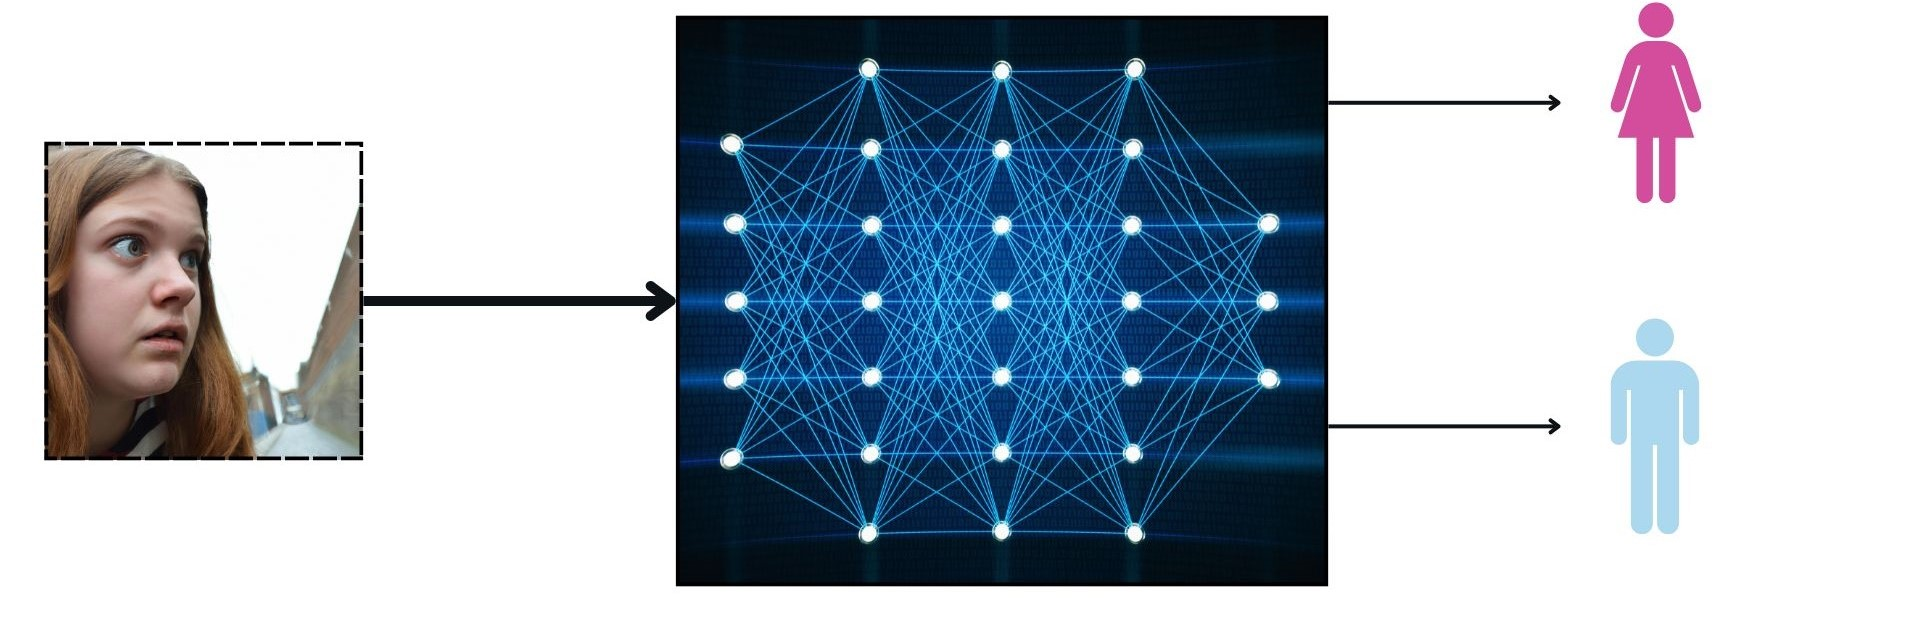
\includegraphics[width=0.85\textwidth]{imgs/CNN_eg.jpg}
\caption{Example Usage of Convolutional Neural Networks for Gender Classification }\label{fig:CNN_example}
\end{figure}

\noindent Before diving into the details of CNNs, let's start with the basics: What is an image to a computer, and what are computer vision tasks?

CNN (သို့မဟုတ်) Convolutional Neural Network သည် visual data / image များနှင့် သက်ဆိုင်သည့် လုပ်ငန်းများကို ဆောင်ရွက်နိုင်ရန်အတွက် ရည်ရွယ်တည်ဆောက်ထားသည့် deep learning architecture များ ဖြစ်သည်။ CNN ကို ဓါတ်ပုံ တစ်ခု ပေးလိုက်ပါက ပုံကို အမျိုးအစား ခွဲခြားပေးနိုင်ခြင်း ၊ ပုံတွင်ပါ၀င်သည့်အရာများကို အုပ်စုဖွဲ့ပေးနိုင်ခြင်း တို့ကို အလိုအလျောက်လုပ်ဆောင်ပေးနိုင်သည်။ Figure \ref{fig:CNN_example}  တွင် CNN ကို အသုံးပြု၍ ဓါတ်ပုံတစ်ပုံအား ကျား/မ ခွဲခြားခြင်းကို ပြသထားသည်။ Support Vector Machine (SVM), Logistic Regression စသည့် Classifier များနှင့် နှိုင်းယှဥ်လျှင် CNN သည် data pre-processing လုပ်ရသည့်အပိုင်းကို အများကြီးလျော့ချပေးနိုင်သည်။ 

\section{Understanding Images and Computer Vision Tasks}

\subsection{What is an image to a computer?}

To a computer, an image is represented as a grid of pixels. Each pixel is the smallest unit of the image and contains information about color and intensity. The structure of an image in a computer can be broken down into:
\begin{itemize}
  \item Grayscale Images: These images are represented by a 2D array where each element corresponds to a pixel. The value of each pixel ranges from 0 (black) to 255 (white). 
\begin{figure}[H]
    \centering
    \begin{minipage}{0.45\textwidth}
        \centering
        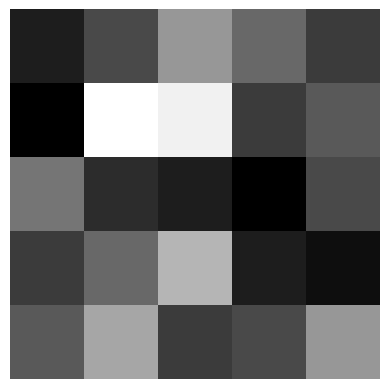
\includegraphics[width=0.4\textwidth]{imgs/grayimg.png}                
    \end{minipage}\hfill
    \begin{minipage}{0.45\textwidth}
        \centering
        \[
        \begin{bmatrix}
            34  &  67  & 123 &  89 &  56 \\
            12  & 200 & 189 &  56 &  78 \\
            98  &  45 &  34 &  12 &  67 \\
            56  &  89 & 145 &  34 &  23 \\
            78  & 134 &  56 &  67 & 123 \\
        \end{bmatrix}
        \]
    \end{minipage}
    \caption{Example of a gray image and its representation in computer}
    \label{fig:gray_img}
\end{figure}
  \item Colored Images: These images are represented by three 2D arrays, each corresponding to one of the color channels: Red, Green, and Blue (RGB). Each pixel is thus represented by a triplet of values, such as (R, G, B), where each value ranges from 0 to 255. 
      \begin{figure}[h]%
        \centering
        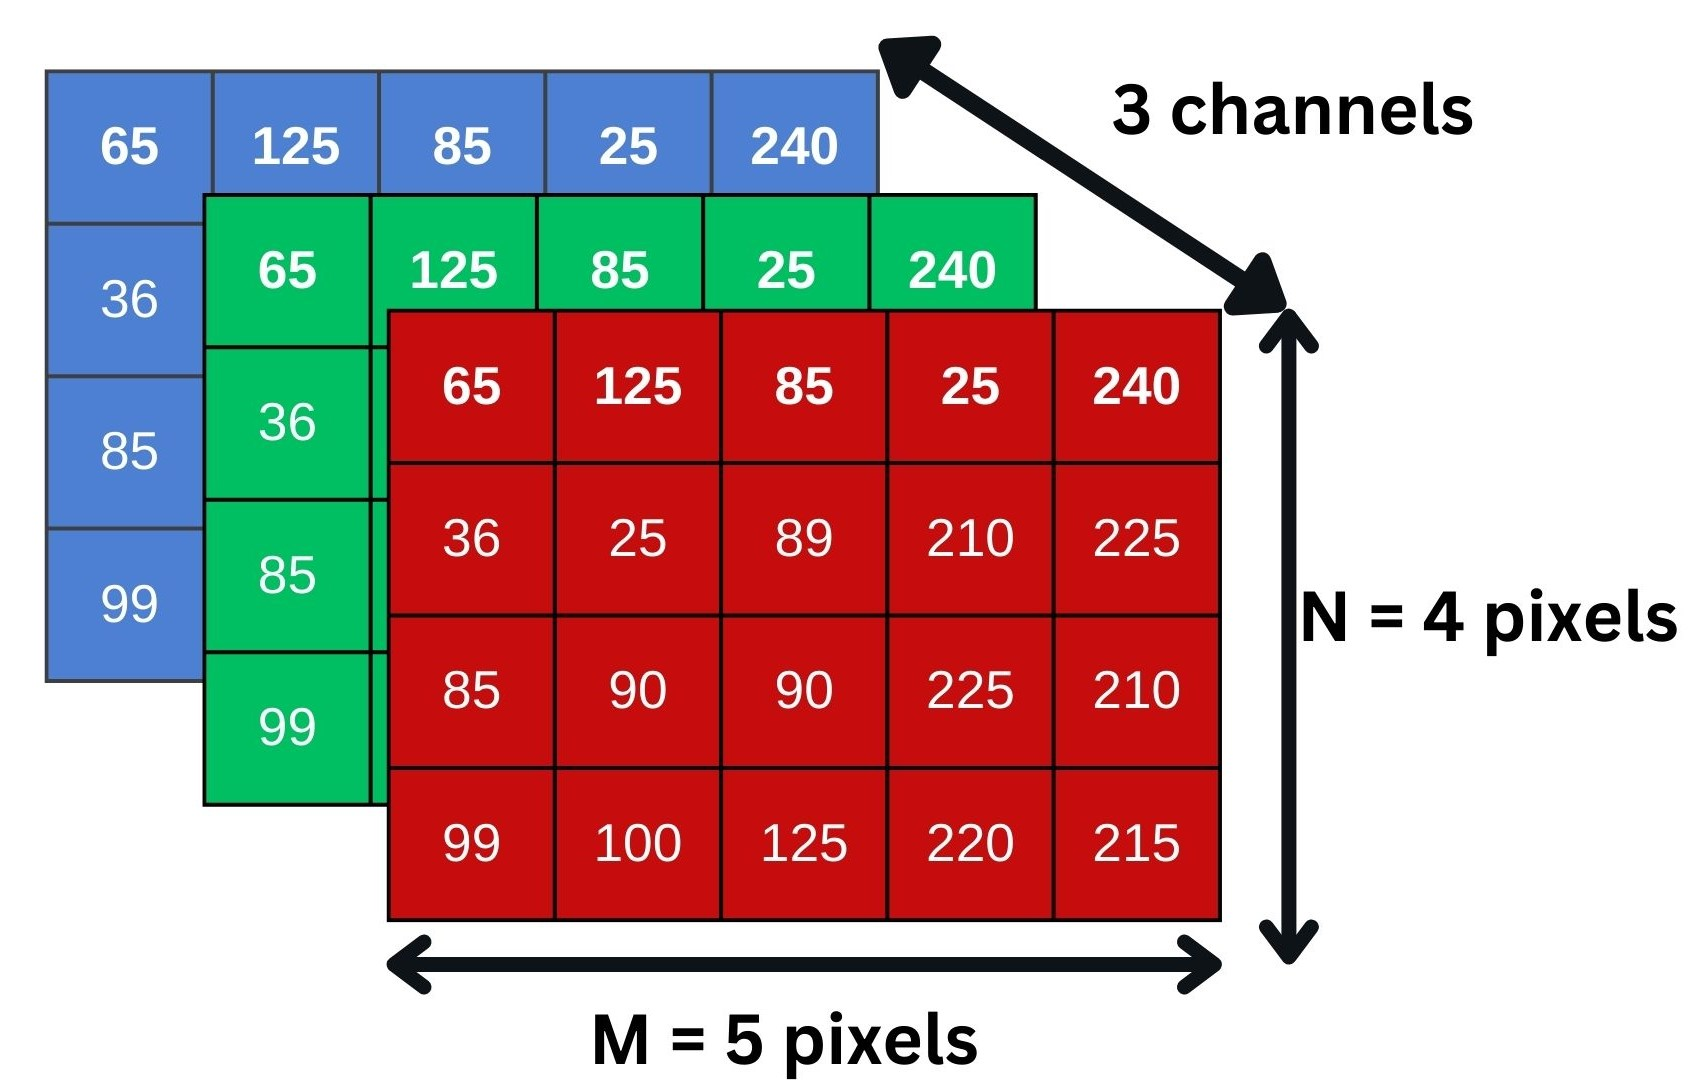
\includegraphics[width=0.75\textwidth]{imgs/colorImg.jpg}
        \caption{Representation of a color image with the resolution of 5 x 4. }\label{fig:colorImg}
        \end{figure}
\end{itemize}

Digital image တစ်ခုကို ကွန်ပြူတာတွင် ဖော်ပြရာ၌ ပုံ (\ref{fig:gray_img} - ဘယ်ဘက်) တွင် ဖော်ပြထားသော အဖြူအမည်း Image မျိုးဖြစ်ပါက pixel တစ်ခုချင်းစီ၏ intensity တန်ဖိုးများကို အသုံးပြုသည်။ pixel တစ်ခုချင်းစီ၏ intensity တန်ဖိုးသည် အဆိုပါ pixel နေရာ၏ အရောင်နှင့် အလင်းကို ဖော်ပြနိုင်သည်။ အဖြူရောင်ကို တန်ဖိုး အများဆုံး ဖြစ်သည့် -၂၅၅ ဖြင့်ဖော်ပြပြီး အနက်ရောက်ကို သုည အဖြစ် သိမ်းဆည်းသည်။ ဥပမာ -- ပုံ (\ref{fig:gray_img} - ဘယ်ဘက်) ၏ ဒုတိယ row ၏ အလယ် pixel နှစ်ခုသည် အခြား   pixel များထက် သိသိသာသာဖြစ်နေသည်ကို တွေ့နိုင်သည်။ ၄င်း  pixel နှစ်ခု၏ တန်ဖိုးကို  ပုံ(\ref{fig:gray_img} - ညာဘက်)ရှိ  matrix တွင်ကြည့်မယ်ဆိုပါက ၂၀၀ နှင့် ၁၈၉ ရှိသည်ကို တွေ့နိုင်သည်။ အခြား အမည်းရောင်ဘက်သို့ သွားသော pixel များ၏ တန်ဖိုးများမှာ နှစ်ဆယ်၊ သုံးဆယ် စသည့်ဖြင့် တစ်ရာ မကျော်သော ကိန်းဂဏန်းများဖြစ်သည်ကို တွေ့ရမည်။ 

Colored Image များကို ကွန်ပြူတာတွင် ဖော်ပြရာ၌ ပုံ (\ref{fig:colorImg}) တွင် ပြသထားသည့် အတိုင်း 3D-matrix ကို အသုံးပြုသည်။ Pixel တစ်ခု၏ color တန်ဖိုးကို Red, Green, Blue Channel များ အသုံးပြု၍ ဖော်ပြရာ အနီရောင် Pixel တစ်ခု၏ တန်ဖိုးမှာ [၂၅၅, ၀, ၀] ဖြစ်ပြီး အပြာရောင် Pixel တစ်ခု၏ တန်ဖိုးမှာ [၀, ၀, ၂၅၅] ဖြစ်မည်။ 

\subsection{Computer Vision Tasks}

Computer Vision is a field of artificial intelligence that enables computers to interpret and make decisions based on visual data from the world. Common tasks in computer vision include:

\begin{enumerate}
    \item \textbf{Image Classification}: Identifying the category or class of an object in an image. For example, recognizing whether an image contains a cat or a dog.
    \item \textbf{Object Detection}: Identifying and locating objects within an image, often by drawing bounding boxes around them. For instance, finding all the cars in a street image.
    \item \textbf{Segmentation}: Dividing an image into multiple segments or regions to simplify analysis. For example, segmenting a scene into trees, buildings and streets, etc. 
    \item \textbf{Biometric Recognition}: Identifying or verifying a person from an image by analyzing biometric features such as fingerprint and faces.
    \item \textbf{Pose Estimation}: Determining the pose of a human body or an object in an image, such as identifying the position and orientation of a person.
    \item \textbf{Optical Character Recognition (OCR)}: Converting different types of documents, such as scanned paper documents or images taken by a digital camera, into editable and searchable data.
    \item \textbf{Image Generation}: Creating new images from scratch or modifying existing images, such as in the case of Generative Adversarial Networks (GANs).
\end{enumerate}

Computer Vision သည် artificial intelligence (AI) လောက၏ အရေးကြီးသော အစိတ်အပိုင်း တစ်ခု ဖြစ်သည်။ ဓါတ်ပုံနှင့် ဗွီဒီယိုများကို ကွန်ပြူတာမှ လူများ နားလည်သကဲ့သို့ နားလည်နိုင်ရန် ထိုဓါတ်ပုံများကို ကြည့်၍ ဆုံးဖြတ်ချက်ချနိုင်ရန် သင်ပေးရသော ဘာသာရပ် တစ်ခုဖြစ်သည်။ Computer Vision ၏ လုပ်ငန်းအချို့မှာ -- 
\begin{itemize}
    \item \textbf{Image Classification}: Image တစ်ခုတွင် ပါ၀င်သည့် object ကို အမျိုးအစား ခွဲခြားပေးခြင်း။  ဥပမာ - လူတစ်ယောက်၏ ဓါတ်ပုံတစ်ပုံကို ပေးလိုက်ပါက Computer Vision Model မှ ကျား/မ ခွဲခြားပေးခြင်းသည် Image Classification / recognition ဖြစ်သည်။ 
    \item \textbf{Object Detection}: Image တစ်ခုတွင် ပါ၀င်သည့် object ကို ရှာဖွေပေးခြင်း။ ဥပမာ -- လမ်းမပေါ်ရှိ ကားများကို detect လုပ်ခြင်း။ 
    \item \textbf{Segmentation}: Image တစ်ခုကို မျိုးတူရာ အုပ်စု ခွဲခြားပေးခြင်း။ ဥပမာ -- Google Map မှ မြင်ရသော ပုံကို လမ်းများ၊ ကားများ၊ သစ်ပင်များ စသည်ဖြင့် တူရာ ခွဲခြားပေးခြင်း။ 
    \item \textbf{Biometric Recognition}:  လက်ဗွေရာ၊ မျက်နှာ စသည့် Biometric features များကို အသုံးပြု၍ လူတစ်ယောက်၏ identity ကို စစ်ဆေးခြင်း။ 
    \item \textbf{Pose Estimation}: လူတစ်ယောက်၏ Pose ကို ခန့်မှန်းခြင်း။ ဥပမာ -- သက်ကြီးရွယ်အိုများ လဲကျသည့် Pose ကို ခန့်မှန်းခြင်း။ 
    \item \textbf{Optical Character Recognition (OCR)}: Scanned ဖတ်ပြီး ရလာသည့် စာသားများကို Recognize လုပ်ပေးခြင်း။ 
    \item \textbf{Image Generation}: စာသား၊  အသံ (သို့မဟုတ်) ပုံရိပ်ဟောင်းများကို အသုံးပြု၍ ပုံရိပ်အသစ်များ တီထွင်ဖန်တီးခြင်း ။ 
    \end{itemize}

\newpage
\section{Architecture of Convolutional Neural Network}\label{CNN_architecture}

The architecture of a Convolutional Neural Network (CNN) encompasses several key components, each playing a crucial role in the network's ability to learn and make predictions. An example of CNN is given in Figure \ref{fig:CNN}. The Convolutional Layer and the Pooling Layer, together form the i-th layer of a Convolutional Neural Network. The convolution layers focus on learning feature representations, and the pooling layers help in summarizing these features. Depending on the complexities in the images, the number of such layers may be increased for capturing low-level details even further, but at the cost of more computational power. 

\vspace{0.5em}
\begin{figure}[h]%
\centering
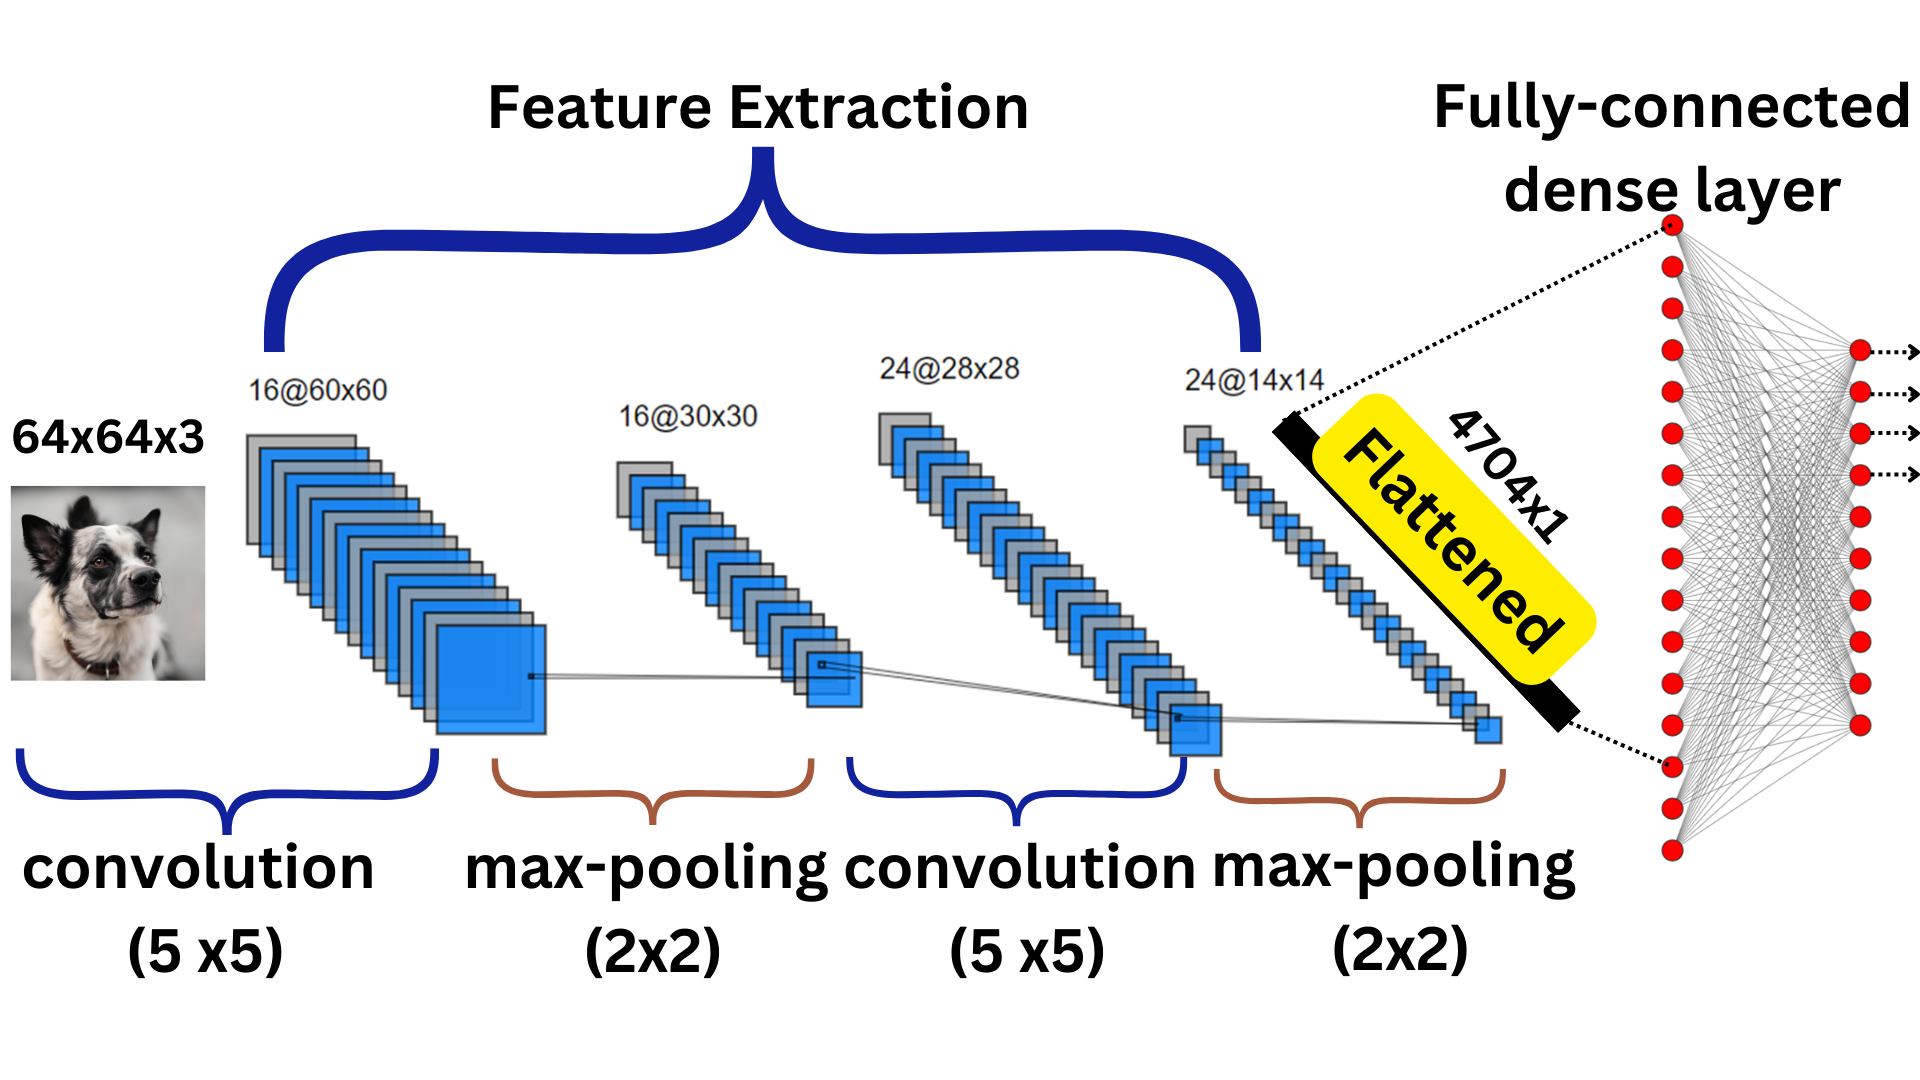
\includegraphics[width=0.8\textwidth]{imgs/cnn_own.png}
\caption{Example of Convolutional Neural Networks.}\label{fig:CNN}
\end{figure}

Integrating the extracted features from convolutional and pooling layers, the fully connected layers establish connections between every neuron in one layer with every neuron in the subsequent layer, similar to traditional neural networks. These layers captures global patterns and relationships within the data, ultimately forming a high-level representation suitable for classification or regression tasks. Notably, the final fully connected layer often serves as the output layer, generating predictions based on the learned features.

CNN  တစ်ခု၏  architecture တွင် အခြေခံအားဖြင့် convolutional, pooling, နှင့် fully connected (dense) layer တို့ ပါ၀င်သည်။ Figure \ref{fig:CNN} တွင် ပြသထားသည့်အတိုင်း Convolution နှင့် Pooling Layer -- ၂ ခု ကို တစ်စုံ အဖြစ် စဥ်းစားနိုင်သည်။ Convolution layer သည် feature များကို ရှာဖွေရန် အဓိက တာ၀န်ယူပြီး Pooling Layer သည် အရေးကြီး သော feature များကို ထုတ်ယူရန် တာ၀န်ယူသည်။ CNN  တစ်ခုတွင် Convolution နှင့် Pooling Layer များစွာ ပါ၀င်နိုင်သည်။  

Fully connected layer သည် ဤ Layer များမှ ရရှိလာသော feature များကို ခြုံငုံချိတ်ဆက်ပေးသည်။           

\subsection{Convolutional Layer}\label{convLayer}

The convolutional layer is a fundamental building block of a CNN. It applies learnable filters, also known as kernels, to the input data using the convolution operation. A kernel (or filter) in the context of convolution is a small matrix that moves over the input data and performs element-wise multiplications followed by a summation to produce a single output value. This process is repeated across the entire input, producing a feature map (or activation map).

\noindent Consider a simple 5x5 grayscale image and a 3x3 kernel given below:
\[
\begin{array}{cc}
\text{Grayscale Image:} & \text{Kernel Matrix:} \\
\begin{bmatrix}
    34  &  67  & 123 &  89 &  56 \\
    12  & 200 & 189 &  56 &  78 \\
    98  &  45 &  34 &  12 &  67 \\
    56  &  89 & 145 &  34 &  23 \\
    78  & 134 &  56 &  67 & 123 \\
\end{bmatrix} & 
\begin{bmatrix}
    1 & 0 & -1 \\
    1 & 0 & -1 \\
    1 & 0 & -1 \\
\end{bmatrix}
\end{array}
\]

The process of convolution involves moving the kernel across the input image and performing element-wise multiplication followed by summation at each location. For instance, at the very first location, the kernel will be multiplied with the pixel intensities highlighted in yellow. The element-wise multiplication and sum will produce the convolution result of 
\begin{equation}\label{eqn:convEg}
(34+12+98)+(0+0+0)-(123+189+34) =-202
\end{equation}

The result of this calculation is the value for the first position of the output matrix, highlighted in the Feature Map (right). Then, the kernel is moved to the next position (in this example, moved by Stride = 1 pixel) and the process is repeated for the entire input image, leading to the resulting matrix:

\[
\begin{array}{cc}
\text{Grayscale Image:} & \text{Convoluted Results (Feature Map)} \\
\begin{bmatrix}
    \colorbox{yellow}{$34$}  &  \colorbox{yellow}{$67$}  & \colorbox{yellow}{$123$} &  89 &  56 \\
    \colorbox{yellow}{$12$}  & \colorbox{yellow}{$200$} & \colorbox{yellow}{$189$} &  56 &  78 \\
    \colorbox{yellow}{$98$}  &  \colorbox{yellow}{$45$} &  \colorbox{yellow}{$34$} &  12 &  67 \\
    56  &  89 & 145 &  34 &  23 \\
    78  & 134 &  56 &  67 & 123 \\
\end{bmatrix} & 
\begin{bmatrix}
    \colorbox{yellow}{$-202$} & 155 & 145 \\
    -202 & 232 & 200 \\
    -3 & 155 & 22 \\
\end{bmatrix}
\end{array}
\]

The size of the feature map (or output) generated by a convolutional layer in a Convolutional Neural Network (CNN) is generally smaller than the input size. This reduction in size depends on several factors, including the kernel size, stride length, and whether padding is applied. In the above example, for a 3x3 kernel with a stride length of 1 and no padding, the feature map produced will be smaller, typically by 2 pixels in each dimension. So, if the input is, for instance, a 64x64 image, the resulting feature map will be 62x62.

The kernel used in the convolution operation determines the types of features detected. The provided kernel function in the above example detects the vertical edges in the image, meaning the pixels where there are vertical edges will have high intensity values in the convolved image. In traditional image processing, kernels are defined by the programmer, and some commonly used kernels include:
\begin{enumerate}
\item \textbf{Laplacian Kernel}: This kernel is employed for edge detection and highlighting areas of rapid intensity change.
\item \textbf{Edge Detector (Sobel Filter)}: It's utilized for detecting edges in specific directions.
\item \textbf{Average Kernel (Box Filter)}: This kernel is applied for blurring or smoothing the image.
\end{enumerate}

However, in Convolutional Neural Networks (CNNs), each convolutional layer employs multiple filters to create multiple feature maps. These filters are initialized randomly and then adjusted during training to minimize the loss function. This adjustment process allows the filters to learn to detect various features automatically, such as edges, patterns, and complex structures, making CNNs highly effective for tasks like image classification and object detection.

Convolutional layer သည် CNN  architecture ၏ အရေးကြီးသော အစိတ်အပိုင်း တစ်ခု ဖြစ်သည်။ ဤ layer တွင် filter (kernel) များကို အသုံးပြု၍ image (input data) တွင် ပါ၀င်သည့် အရေးကြီးသော feature များကို ရှာဖွေသည်။ ဤနေရာတွင် kernel ဆိုသည်မှာ k x k matrix တစ်ခုသာ ဖြစ်သည်။ အထက်တွင် 3 x 3 kernel နမူနာ တစ်ခုကို ဖော်ပြထားသည်။ Convolution ပြုလုပ်သည် ဆိုခြင်းမှာ အဆိုပါ kernel ကို image တလျောက် နေရာရွေ့၍  kernel နှင့် input data ကို မြှောက်၍ ပေါင်းလဒ်ကို ရှာဖွေခြင်း ဖြစ်သည်။ 

အထက်ပါ ဥပမာ ကို ကြည့်မည်ဆိုပါက feature map ၏ ပထမဆုံး တန်ဖိုးသည် image ၏ ပထမဆုံး pixel ကိုးခုနှင့် kernel ၏ တန်ဖိုးများကို မြှောက်၍ စုစုပေါင်းတန်ဖိုး  ($(34+12+98)+(0+0+0)-(123+189+34) =-202$) ကို ရှာဖွေခြင်း ဖြစ်သည်။ ယခု ဥပမာ တွင် အသုံးပြုထားသည့် kernel သည် ဒေါင်လိုက် Line များကို ရှာဖွေရာတွင် အသုံးပြုနိုင်သည်။ image processing များ ပြုလုပ်ရာတွင် ဒေါင်လိုက်၊ အလျားလိုက်နဲ့ ဒေါင့်ဖြတ်ဖြစ်နေသာ လိုင်းများကို ရှာဖွေပေးသည့် အထက်ပါ Edge Detector များအပြင် ပျမ်းမျှ တန်ဖိုးကို ရှာဖွေပေးသော Average Kernel များ ၊ ရုတ်တရက် intensity တန်ဖိုးပြောင်းသွားသည့် Edge ကို ရှာဖွေပေးသည့် Laplacian Kernel များကိုလည်း အသုံးပြုကြသည်။ 

သို့သော် CNN တွင်မူ convolutional layer တစ်ခုတွင် filter တစ်ခုမက အသုံးပြုပြီး filter ကို ကြိုတင်သတ်မှတ်ထားရန် မလိုအပ်ပါ။ Training ပြုလုပ်ရာတွင် loss (input output ကြား ကွာခြားချက်) အနည်းဆုံး ဖြစ်စေမည့် filter ကို Optimization algorithm များ အသုံးပြု၍ ရှာဖွေသည်။ ထိုသို့ရှာဖွေဖြင်းဖြင့် image များကို အမျိုးအစားခွဲခြားခြင်း ၊ object ကို ရှာဖွေခြင်း စသည့် task များအတွက် အသုံး၀င်မည့် feature များကို ရရှိပြီး CNN ၏ Performance ကို ပိုမို ကောင်းမွန်စေသည်။ 


\subsection{Pooling Layer}\label{poolLayer}
The pooling layer serves to decrease the spatial dimensions of feature maps while retaining crucial information. Common pooling operations include max pooling and average pooling, which aid in achieving translation invariance and computational efficiency. There are two primary types of pooling: Max Pooling and Average Pooling.

\vspace{0.5em}
\begin{figure}[h]%
\centering
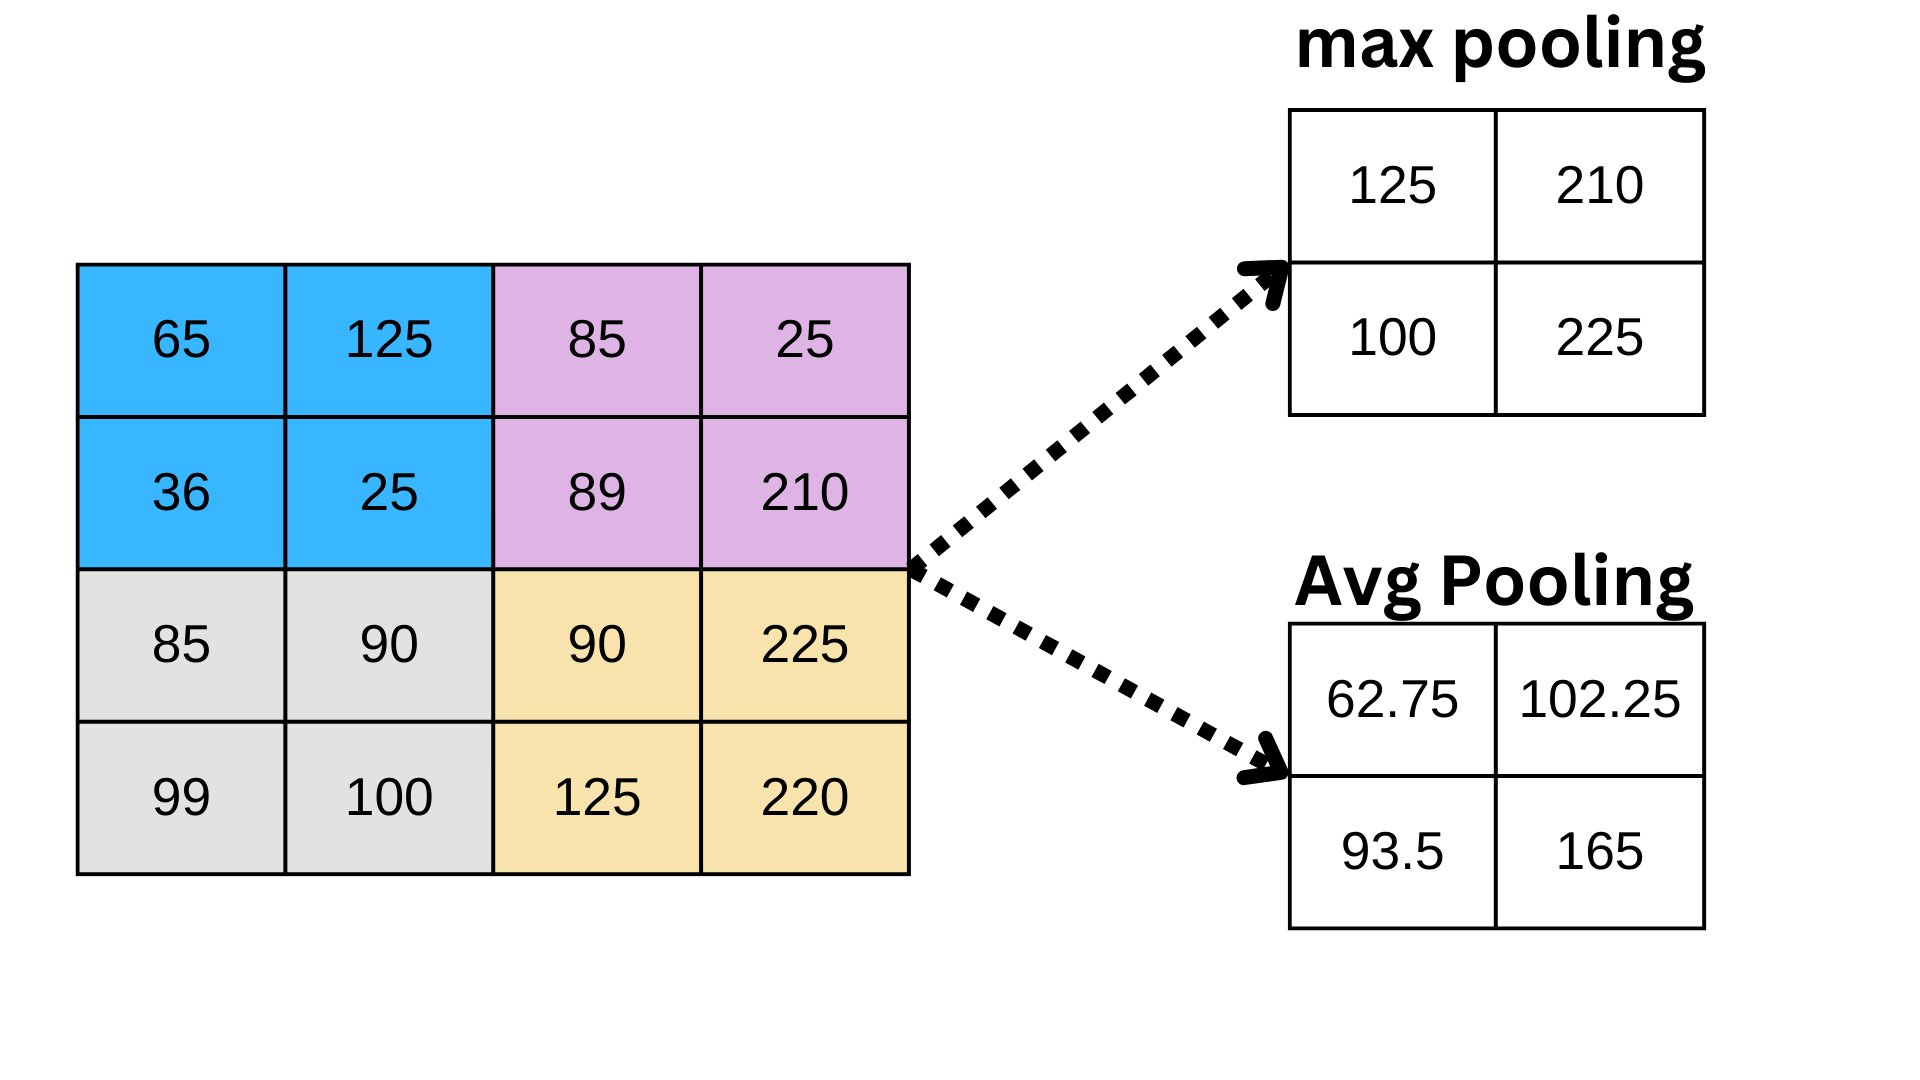
\includegraphics[width=0.75\textwidth]{imgs/cnn_pool.png}
\caption{Example of max-pooling and average pooling.}\label{fig:CNNPooling}
\end{figure}

Max Pooling selects the maximum value from the section of the image covered by the kernel, whereas Average Pooling computes the average of all the values within the kernel's coverage area. In Figure \ref{fig:CNNPooling}, the operation of both max pooling and average pooling on a 4x4 convoluted image is illustrated.

By utilizing a 2x2 kernel in the pooling layer, the size of the input data is halved. For example, if the input (convoluted map) is a 62x62 image, the resulting matrix will be reduced to 31x31.


\subsection{Fully Connected Layer}\label{FCLayer}
Once the convolutional and pooling layers have extracted important features, the model proceeds to a fully connected layer. Here, the final output from these layers is flattened and fed into a traditional feed-forward neural network for classification or regression tasks.

The fully connected layer learns non-linear combinations of the high-level features represented by the output of the convolutional and pooling layers. Through forward and backpropagation, the feed-forward neural network adjusts its parameters to understand the complex relationships within the data. Over multiple epochs, the model distinguishes between dominant and subtle features in the images, utilizing an appropriate activation function to produce the output.

The choice of activation function in the output layer depends on the task at hand. For binary classification, a sigmoid activation function is often chosen, while for multi-class classification, a softmax activation function is commonly used. In regression tasks, the output layer typically comprises a single neuron with a linear activation function, generating a continuous output value.

Fully Connected Layer သည် ပြီးခဲ့သည့် အခန်းတွင် ရှင်းပြခဲ့သည့် Feed-forward neural network ၏ hidden layer (သို့မဟုတ်) output layer များနှင့် သဘောတရားအတူတူပင် ဖြစ်သည်။ Convolution နှင့် Pooling Layer များမှ အရေးကြီးသည့် features များကို သင်ယူပြီးနောက် ဤ Layer များ၏ final output မှာ feature vector တစ်ခု ဖြစ်သည်။  အဆိုပါ feature vector သည်  Feed-forward neural network (MLP) ၏ input vector ဖြစ်မည်။ ထို့နောက် MLP မှ forward နှင့် backward propagation ကို ကြိမ်ဖန်များစွာ ပြုလုပ်ပြီး model အတွက် လိုအပ်သည့် parameters များကို Feature (training set) မှ ရှာဖွေမည် ဖြစ်သည်။ 

Feed-forward neural network တွင် Fully Connected hidden layer တစ်ခု (သို့မဟုတ်)နှစ်ခု နှင့် output layer တစ်ခုတို့ ပါ၀င်သည်။ နောက်ဆုံး Fully Connected output layer တွင် အသုံးပြုမည့် activation function သည် လုပ်ဆောင်မည့် လုပ်ငန်းပေါ်တွင် မူတည်၍ ရွေးချယ်ရမည်။ အမျိုးအစား ၂ ခု ကိုသာ ခွဲခြားပေးသော Binary Classification ပုစ္ဆာများတွင် sigmoid activation function ကို အသုံးပြုပြီး multi-class classification တွင်မူ softmax activation function ကို အသုံးပြုကြသည်။ Output Layer တွင် ပါ၀င်ရမည့် unit (neuro) မှာ ခွဲခြားပေးရမည့် Output အရေအတွက်ပေါ်တွင် မူတည်သည်။ ဥပမာ -- ခွေး(သို့မဟုတ်) ကြောင် ဟု ခွဲခြားပေးမည့် Classifier ၏ Output Layer ရှိ unit (neuro) အရည်အတွက်မှာ ၂ ဖြစ်ပြီး လက်ရေးဖြင့်ရေးထားသော number များကို ခန့်မှန်းမည့် Classifier အတွက်မူ unit (neuro) အရည်အတွက် တစ်ဆယ် (သုညမှ ၉ အထိ) ဖြစ်ရမည်။ Regression အတွက်မူ unit (neuro) တစ်ခုသာ ပါ၀င်ပြီး linear activation function ကို အသုံးပြုသည်။ 

\setcounter{stepcounter}{0}
\subsection{Building a CNN Architecture}
This section gives an example of how to build a Convolutional Neural Network (CNN) architecture using the `keras` library in Python. The model is structured as a sequential model, integrating multiple convolutional layers, max-pooling layers, a flattening layer, and fully connected layers, as demonstrated in Figure \ref{fig:CNNArch}.

ဤအခန်းတွင် Convolutional Neural Network (CNN) architecture တစ်ခုကို `keras` library အသုံးပြုပြီး တည်ဆောက်ပြထားခြင်း ဖြစ်ပါသည်။ Python ကုဒ်များဖြစ်သည့်အတွက် မြန်မာဘာသာ ပြန်ဆိုခြင်း မပြုထားပါ။ စာဖတ်သူများအနေဖြင့် ပေးထားသည့် GitHub Repo ကို Fork လုပ်၍ Python ကုဒ်များကို တစ်ကြောင်းချင်း run ကြည့်ရန် အကြံပြုပါသည်။ ဤ architecture တွင် convolutional layer သုံးစုံ၊ flattening layer တစ်ခုနှင့် fully connected layer နှစ်ခုတို့ ပါ၀င်ရာ layer တစ်ခုချင်းစီကို architecture ထဲသို့ မည်သို့ ထည့်ရမည်ကို အဆင့် (၅) ဆင့်ဖြင့် ရှင်းလင်းပြထားပါသည်။ ပါ၀င်သည့် layer တစ်ခုချင်းစီအတွက် လိုအပ်သည့် parameter အရည်အတွက်များကို နောက်အခန်းတွင် အသေးစိပ် ရှင်းပြသွားမည်။ 

\vspace{0.5em}
\begin{figure}[h]%
\centering
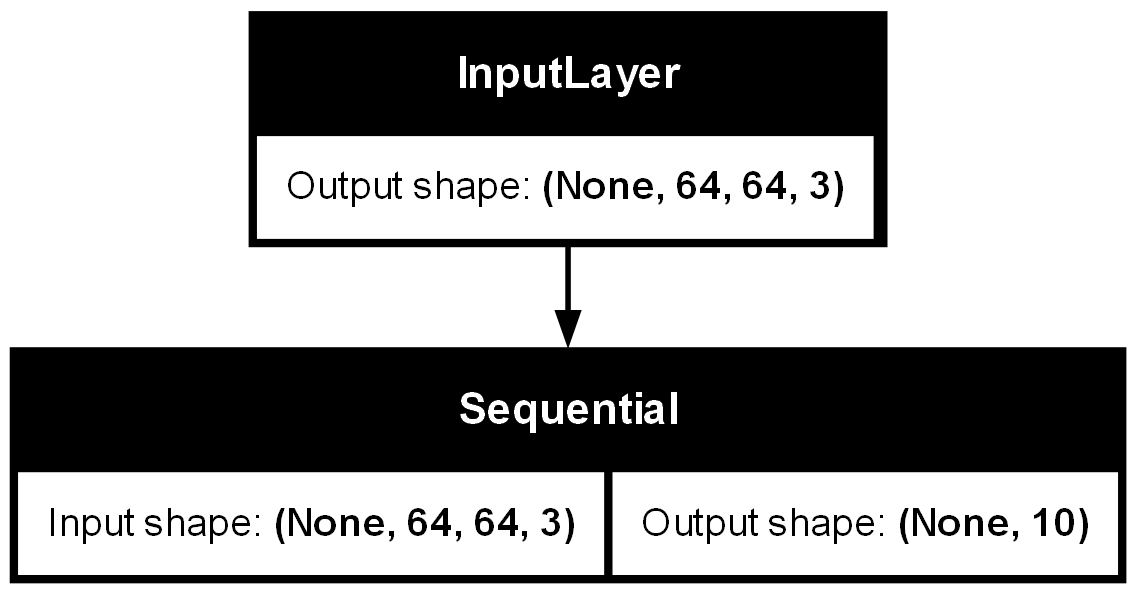
\includegraphics[width=0.55\textwidth]{imgs/cnn_model_seq.png}
\caption{Example of CNN Model Architecture}\label{fig:CNNArch}
\end{figure}

\begin{step}
First, an input layer is defined to specify the shape of the input data. In general, the shape of the input data is the size of the image. 
\begin{verbatim}
inputs = Input(shape=input_shape)
\end{verbatim}
\end{step}

\begin{step}
A Sequential model is then, constructed to define the architecture of the CNN.
\begin{verbatim}
model = Sequential()
\end{verbatim}
\end{step}
\begin{step}
In this step, three convolutional layers, each comprising a convolutional layer followed by a max-pooling layer, are added to the sequential model defined in Step 2.
\paragraph*{Convolutional Layer 1}
\begin{itemize}
    \item \texttt{Conv2D}: 32 filters, kernel size of 5x5, activation function \texttt{relu}.
    \item \texttt{MaxPooling2D}: Pool size of 2x2.
\end{itemize}
\begin{verbatim}
model.add(Conv2D(32, (5, 5), activation='relu'))
model.add(MaxPooling2D((2, 2)))
\end{verbatim}

\paragraph*{Convolutional Layer 2}
\begin{itemize}
    \item \texttt{Conv2D}: 64 filters, kernel size of 5x5, activation function \texttt{relu}.
    \item \texttt{MaxPooling2D}: Pool size of 2x2.
\end{itemize}
\begin{verbatim}
model.add(Conv2D(64, (5, 5), activation='relu'))
model.add(MaxPooling2D((2, 2)))
\end{verbatim}

\paragraph*{Convolutional Layer 3}
\begin{itemize}
    \item \texttt{Conv2D}: 128 filters, kernel size of 5x5, activation function \texttt{relu}.
    \item \texttt{MaxPooling2D}: Pool size of 2x2.
\end{itemize}
\begin{verbatim}
model.add(Conv2D(64, (5, 5), activation='relu'))
model.add(MaxPooling2D((2, 2)))
\end{verbatim}
\end{step}

\begin{step}
In Step 4, the output from the convolutional layers undergoes flattening, transforming the 2D matrix data into a 1D vector. This flattened representation is then fed into two fully connected layers. Finally, the last layer serves as the output layer, containing 10 labels.

\paragraph*{Flattening Layer} 
\begin{verbatim}
model.add(Flatten())
\end{verbatim}

\paragraph*{Fully Connected Layer}
\begin{itemize}
    \item \texttt{Dense}: 512 units, activation function \texttt{relu}.
    \item \texttt{Output layer}: 10 units (assuming 10 classes for classification), activation function \texttt{softmax}.
\end{itemize}
\begin{verbatim}
model.add(Dense(512, activation='relu'))
model.add(Dense(10, activation='softmax'))
\end{verbatim}
\end{step}

\begin{step}
Finally, the model is built by specifying the inputs and outputs.
\begin{verbatim}
model = Model(inputs=inputs, outputs=model(inputs))
\end{verbatim}
\end{step}

\subsection{Parameter Analysis}
The total number of trainable parameters in a CNN model significantly impacts its capacity and performance. These parameters are influenced by factors such as the size of convolutional filters, the number of filters in each layer, and the dimensions of fully connected layers.

\begin{table}[htbp]
    \centering    
    \caption{Summary of CNN Model Architecture}
    \label{tab:cnnR}
    \begin{tabular}{|l|l|l|}
    \hline
    \textbf{Layer (type)}             & \textbf{Output Shape}   & \textbf{Param \#} \\
    \hline
    input\_layer\_2 (InputLayer)      & (None, 64, 64, 3)       & 0                 \\
    \hline
    conv2d\_3 (Conv2D)                & (None, 60, 60, 32)      & 2,432             \\
    \hline
    max\_pooling2d\_3 (MaxPooling2D)  & (None, 30, 30, 32)      & 0                 \\
    \hline
    conv2d\_4 (Conv2D)                & (None, 26, 26, 64)      & 51,264            \\
    \hline
    max\_pooling2d\_4 (MaxPooling2D)  & (None, 13, 13, 64)      & 0                 \\
    \hline
    conv2d\_5 (Conv2D)                & (None, 9, 9, 128)       & 204,928           \\
    \hline
    max\_pooling2d\_5 (MaxPooling2D)  & (None, 4, 4, 128)       & 0                 \\
    \hline
    flatten\_1 (Flatten)              & (None, 2048)            & 0                 \\
    \hline
    dense\_2 (Dense)                  & (None, 512)             & 1,049,088         \\
    \hline
    dense\_3 (Dense)                  & (None, 10)              & 5,130             \\
    \hline
    \end{tabular}
\end{table}

Table \ref{tab:cnnR} provides a breakdown of the parameters for each layer of the CNN model outlined above. The input layer simply defines the shape of the input image and does not have any trainable parameters. Hence, the number of parameters for the input layer is zero. 

The convolutional layers are where CNN learns the features and these layers contribute significantly to the total parameter count. Typically, the number of parameters in a convolutional layer is calculated by multiplying the filter width $m$, by the filter height $n$, by the depth $d$ of the input volume, and the number of filters $k$ in the current layer, and then adding bias terms for each filter. For example, in Convolutional Layer 1, the number of parameters is calculated as $(5 \times 5 \times 3 \times 32) + 32 = 2,432$.

The max-pooling layer does not have any parameters, as it simply selects the maximum value from the input regions and does not involve any learning process. In contrast, the fully connected layers have the highest number of parameters because every neuron in the previous layer is connected to every neuron in the current layer. Hence, the number of parameters is the product of the number of neurons in the current layer $c$ and the number of neurons in the previous layer $p$, plus the bias terms. For example, the number of parameters for the first fully connected layer is calculated as follows: $((c * p)+1*c = 512*2048 + 512 = 1,049,088)$.

The number of parameters in the CNN model directly affects the computational resources required for training and inference. Larger models with more parameters demand higher computational resources and longer training times, making scalability an important consideration in model development and deployment.

CNN model တစ်ခု၏ performance သည် အဆိုပါ model တွင် ပါ၀င်သည့် parameter အရေအတွက် ပေါ်တွင် မူတည်သည်။ အထက်ပါ ဇယားတွင် CNN model တစ်ခု၏ layer အသီးသီးတွင် ပါ၀င်သည့် parameter အရေအတွက်ကို ဖော်ပြထားပြီး တွက်ချက်ပုံ အဆင့်ဆင့်ကို ရှင်းပြသွားမည်။ ဤသင်ခန်းစာတွင် နမူနာပြထားသည့် Model တွင် Input image သည် color image တစ်ခုဖြစ်ပြီး ၄င်း၏ အရွယ်အစားမှာ  $(64 \times  64)$ ဖြစ်သည်။ input layer တွင် parameter ကို တွက်ချက်ရန် မလိုအပ်ပါ။  

Convolutional layer များတွင် လိုအပ်သည့် parameter အရေအတွက်သည် convolutional filter ၏ အရွယ်အစား၊ filter အရေအတွက်များ အပေါ်တွင် မူတည်သည်။ ဥပမာ ဒုတိယ layer တွင်  $(5 \times 5 )$ convolutional filter ကို အသုံးပြုထားပြီး filter အရေအတွက်မှာ သုံးဆယ့်နှစ်ခု ဖြစ်သည်။ထို့ပြင် မူလ Input image တွင် channel သုံးခုပါ၀င်ရာ ဤ convolutional layer တွင် တွက်ချက်ရမည့် parameter အရေအတွက်မှာ $(5 \times 5 \times 3 \times 32) + 32 = 2,432$, နှစ်ထောင့် လေးရာ သုံးဆယ့်နှစ်ခု ဖြစ်သည်။ ထည့်ပေါင်းထားသည့် ၃၂ မှာ filter တစ်ခုချင်းစီအတွက် bias term တစ်ခု စီ ထည့်ပေါင်းထားခြင်း ဖြစ်သည်။ 

max-pooling layer သည် filter အတွင်းရှိ အကြီးဆုံး တန်ဖိုးကို ဆွဲထုတ်ခြင်းသာ ဖြစ်ရာ parameter ကို တွက်ချက်ရန် မလိုအပ်ပါ။  များသောအားဖြင့် CNN model  တွင် parameter အများဆုံးသော layer မှာ fully connected layer များဖြစ်သည်။ fully connected ဟုဆိုသည့်အတိုင်း ပြီးခဲ့သည့် layer ၏ neuron တစ်ခုတိုင်းသည် ယခု layer ၏ neuron တိုင်းနှင့်ချိတ်ဆက်ထားသည် ဖြစ်ရာ parameter အရေအတွက်မှာ  layer နှစ်ခု၏ neuron  အရည်အတွက် မြှောက်ခြင်း ဖြစ်သည်။ ဥပမာ - ယခု နမူနာပြထားသည့် Model ၏ ပထမ fully connected layer တွင် neuron အရေအတွက်မှာ  ငါးရာတစ်ဆယ့်နှစ်ခု ရှိပြီး flattened Layer တွင် ရှိသည့် neuron အရေအတွက်မှာ  နှစ်ထောင့်လေးဆယ့်ရှစ်ခုဖြစ်သည်။ သို့ဖြစ်ရာ ပထမ fully connected layer အတွက်  လိုအပ်သည့် parameter အရေအတွက်မှာ တစ်သန်း လေးသောင်း ကိုးထောင် ရှစ်ဆယ့် ရှစ်ခု $((c * p)+1*c = 512*2048 + 512 = 1,049,088)$ ဖြစ်သည်။ 

CNN model တစ်ခုတွင် တွက်ချက်ရန် လိုအပ်သည့် parameter များလာသည်နှင့် အမျှ model ကို Training ပြုလုပ်ရန် အသုံးပြရသည့် ကြာချိန် ပိုကြာမြင့်လာပြီး computational resource များလည်း ပိုမို လိုအပ်လာသည်။ 

\newpage
\section{Various architectures of CNNs}\label{sec:vCNN}

There are numerous architectures of Convolutional Neural Networks (CNNs), each designed to address different challenges and tasks in the field of computer vision. They are typically different based on the number of layers and activation functions used. In this section, a few backbone CNN architectures are discussed. 

Convolutional Neural Network architecture တွင် အသုံးပြုသည့် activation function အမျိုးအစား၊ convolutional နှင့် fully connected layer အရည်အတွက် ပေါ်တွင် မူတည်၍ Convolutional Neural Network အမျိုးမျိုး ရှိသည်။ ဤအခန်းတွင် လူသုံးများသည့် CNN architecture အချို့ကို ဆွေးနွေးသွားမည်။ 

\subsection{AlexNet}

AlexNet \cite{AlexNet2012} is a convolutional neural network (CNN) architecture that was developed by Alex Krizhevsky, Ilya Sutskever, and Geoffrey Hinton. It won the ImageNet Large Scale Visual Recognition Challenge (ILSVRC) in 2012. The AlexNet architecture consists of eight layers: five convolutional layers, some of which are followed by max-pooling layers, two fully connected hidden layers, and one fully connected output layer.

\vspace{0.5em}
\begin{figure}[h]%
\centering 
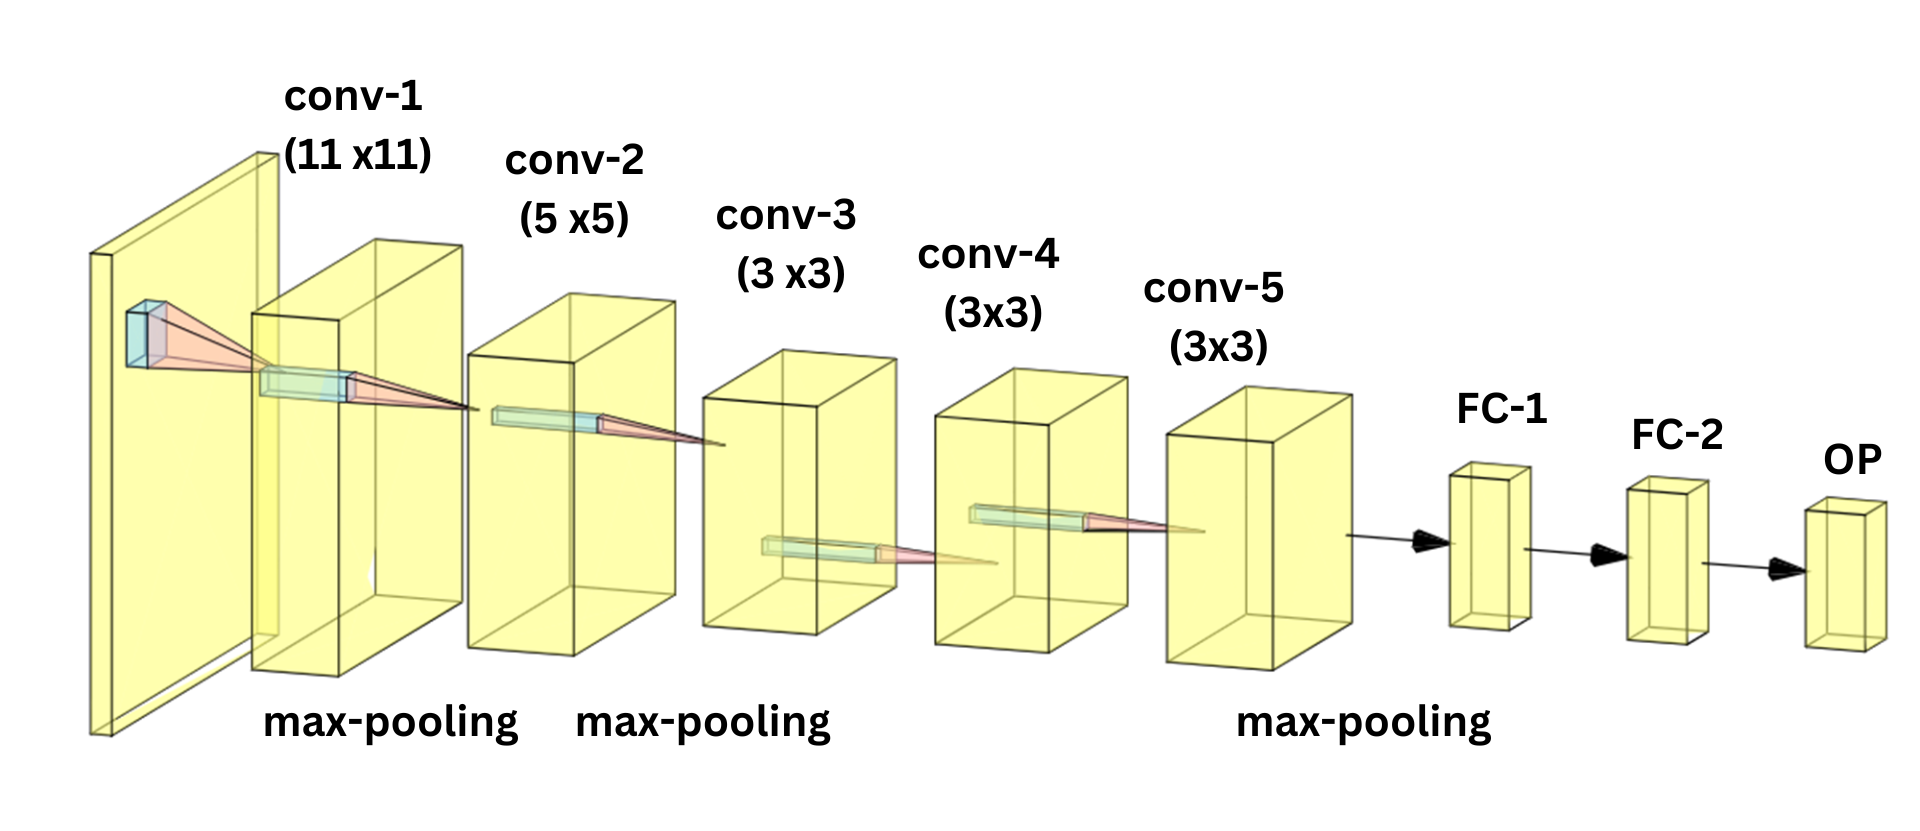
\includegraphics[width=0.75\textwidth]{imgs/alexnet.png}
\caption{AlexNet Architecture. Image created by\cite{web:NNSVG}}\label{fig:alexnet}
\end{figure}

AlexNet သည် Alex Krizhevsky, Ilya Sutskever, နှင့် Geoffrey Hinton တို့ တီထွင်ခဲ့သော convolutional neural network architecture ဖြစ်သည်။ ၂၀၁၂ ခုနှစ် ILSVRC ပြိုင်ပွဲတွင် ဆုရရှိခဲ့သည်။ AlexNet architecture တွင် convolutional layer ၅ ခု ၊ fully connected hidden layer - နှစ်ခုနှင့် output layer - တစ်ခု တို့ပါ၀င်သည်။ အချို့ convolutional layer များတွင် တွဲဖက်ဖြစ်သော max-pooling layer ပါ၀င်သည်။ 

\subsection{VGGNet}

VGGNet \cite{VGGNet2014}  was developed by the Visual Geometry Group (VGG) at the University of Oxford and achieved outstanding performance in the ILSVRC 2014 competition. The architecture is known for its simplicity and depth, consisting of small convolutional filters (3×3) and a very deep network with 16 to 19 layers.

VGGNet primarily comes in two variants based on depth: VGG16, which has 16 layers, and VGG19, which has 19 layers. The architecture typically includes five sets of convolutional layers, each followed by max-pooling layers, and concludes with three fully connected layers. VGGNet uses ReLU activation functions throughout the network and finishes with a softmax classifier for the final output.

\vspace{0.5em}
\begin{figure}[h]%
\centering 
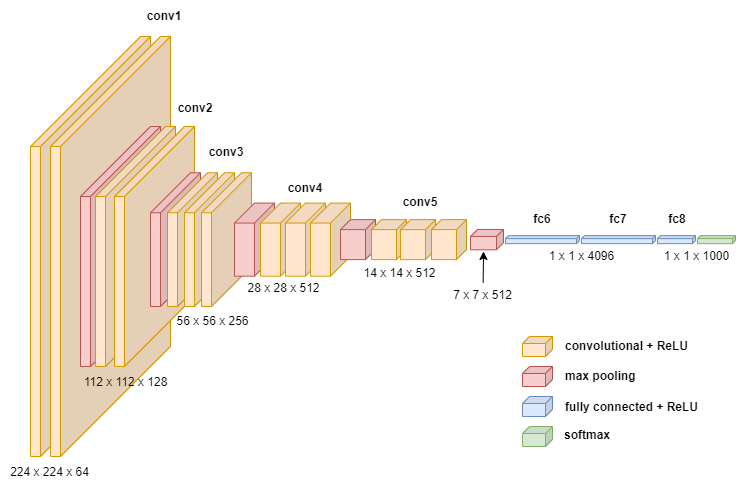
\includegraphics[width=0.75\textwidth]{imgs/vgg16.png}
\caption{VGGNet-16 Architecture. Image Source: \cite{web:NNDiagrams}}\label{fig:vgg-16}
\end{figure}

VGGNet ကို University of Oxford မှ  Visual Geometry Group (VGG) တီထွင်ခဲ့ပြီး ၂၀၁၄ ခုနှစ် ILSVRC ပြိုင်ပွဲတွင် ထူးခြားကောင်းမွန်သည့် ရလဒ်များကို တင်ပြနိုင်ခဲ့သည်။ VGGNet ၏ ထူးခြားချက်မှာ သေးငယ်သော convolutional filter (3x3) ကို အသုံးပြုထားပြီး image ၏ အသေးစိပ် Feature များကို ရှာဖွေခြင်း ဖြစ်သည်။ ထို့အပြင် network တွင် convolutional layer များစွာကို အသုံးပြုသည်။ ယေဘူယျအားဖြင့် VGGNet တွင် convolutional layer အုပ်စု ၅ ခု နှင့် fully connected layer - ၃ ခု တို့ပါ၀င်သည်။  convolutional layer အုပ်စု တစ်ခုတွင် convolutional layer နှစ်ခု (သို့မဟုတ်) သုံးခုအပြင် max-pooling layer တစ်ခုစီလည်း ပါ၀င်သည်။ 

VGGNet architecture တွင် layerတစ်ဆယ့်ခြောက် ခု ပါ၀င်သော VGG16 နှင့် layer တစ်ဆယ့်ကိုးခု ပါ၀င်သော VGG19 ဟု အမျိုးအစား နှစ်မျိုး ရှိသည်။ VGG16 တွင် convolutional layer နှစ်ခု နှင့် max-pooling layer တစ်ခု ပါ၀င်သော အုပ်စု  နှစ်စု၊ convolutional layer သုံးခု နှင့် max-pooling layer တစ်ခု ပါ၀င်သော အုပ်စု  သုံးစု အပြင် fully connected layer - ၃ ခု  ပါ၀င်သည်။ သို့ဖြစ်ရာ VGG16 တွင် ပါ၀င်သည့် စုစုပေါင်း layer အရေအတွက်မှာ (၂ x ၂  + ၃ x ၃ + ၃ = ၁၆) ခု ဖြစ်သည်။ ဤတွက်ချက်မှုတွင် max-pooling layer ကို ထည့်တွက်ခြင်း မပြုထားပါ။ 

\subsection{ResNet (Residual Network)}
ResNet\cite{ResNet_2016}, short for Residual Network, is a type of deep neural network architecture introduced by Kaiming He et al. in 2015. Deep neural networks often suffer from the vanishing gradient problem, where gradients become progressively smaller as they backpropagate from the output layer to the input layer. As a result, earlier layers receive minimal updates, significantly hindering their learning. This problem is common in deep networks, posing a major challenge during training. In addition to vanishing gradients, deep networks can also face the exploding gradient problem, where gradients grow exponentially during backpropagation, leading to model instability. 

\vspace{0.5em}
\begin{figure}[h]%
\centering 
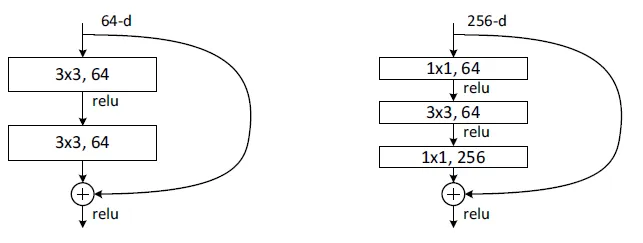
\includegraphics[width=0.85\textwidth]{imgs/res_block.png}
\caption{Residual Blocks. Image Source: \cite{ResNet_2016}}\label{fig:resnet}
\end{figure}

ResNet addresses both the vanishing and exploding gradient problems by introducing shortcut connections, or residual connections, which allow gradients to bypass one or more layers, thereby preserving the gradient flow and stabilizing the training process. The core idea of ResNet is the use of residual blocks (shown in Figure \ref{fig:resnet}), which consist of two or three layers with a direct (shortcut) connection that skips one or more layers. ResNet introduced several versions of the model with varying depths: ResNet-18, ResNet-34, ResNet-50, ResNet-101, and ResNet-152. These models utilize different types of residual blocks to balance between complexity and computational efficiency.

\begin{itemize}[b]
  \item \textbf{Basic Residual Block}(Figure \ref{fig:resnet}-left)), used in ResNet-18 and ResNet-34, consists of 2 layers, typically 3x3 convolutional layers. 
  \item \textbf{Bottleneck Residual Block}(Figure \ref{fig:resnet}-right), used in ResNet-50 and ResNet-101, comprises 3 layers: a 1x1 convolutional layer for dimensionality reduction, a 3x3 convolutional layer, and another 1x1 convolutional layer for restoring the dimensions. 
\end{itemize}

Shallower networks like ResNet-18 and ResNet-34 are faster and less computationally intensive, making them suitable for tasks with limited computational resources. In contrast, deeper networks like ResNet-50 and ResNet-101 can capture more complex patterns, making them better suited for challenging tasks, though they require higher computational resources.

ResNet (သို့မဟုတ်) Residual Network ကို ၂၀၁၅ ခုနှစ်တွင် Microsoft မှ သိပ္ပံပညာရှင် Kaiming He နှင့် အဖွဲ့မှ စတင် တီထွင်ခဲ့ကြသည်။ အထက်တွင် ဆွေးနွေးခဲ့သည့် architecture များကို လေ့လာကြည့်မည် ဆိုပါက model တွင် ပါ၀င်သည့် layer များ ပိုမို များပြားလာသည်နှင့် အမျှ အဆိုပါ architecture ၏ စွမ်းဆောင်ရည်သည် မြင့်တက်လာသည်။ သို့သော် ထိုသို့ layer များ ပိုမိုများလာသည်နှင့်အမျှ parameter များကို update လုပ်သည့် backpropagate လုပ်ငန်းစဥ်တွင် အသုံးပြုသည့် gradient တန်ဖိုးမှာ သေးသည်ထက် သေးလာခြင်း (သို့မဟုတ်) အဆမတန် ကြီးမားလာတတ်သည်။ ဤ ပြဿနာကို  vanishing/exploding gradient problem ဟု ခေါ်ဆိုကြသည်။ ထိုပြဿနာမျိုး ဖြစ်လာပါက အချို့ parameter များသည် တန်ဖိုးမပြောင်းလဲတော့ခြင်း ( gradient တန်ဖိုး သေးလာပါက)၊  အချို့ parameter များ၏ တန်ဖိုးသည် အဆမတန်ကြီးလာနိုင်သည်။ အကျိုးဆက်အားဖြင့် model ၏ စွမ်းဆောင်ရည်များ ကျလာသည်။ 

ResNet သည် အထက်ပါ ပြဿနာများကို ဖြေရှင်းနိုင်ရန်အတွက်  shortcut connection ဟုခေါ်ဆိုသည့် အိုင်ဒီယာ အသစ်တစ်ခုကို တီထွင်ခဲ့ကြသည်။  shortcut connection သည် အချို့ layer များကို အစီအစဥ်အလိုက် မချိတ်ဆက်ဘဲ နှစ်ခု (သို့မဟုတ်) သုံးခုကို ကျော်၍ ချိတ်ဆက်ခြင်းမျိုး ဖြစ်သည်။ ထိုသို့ကျော်၍ ချိတ်ဆက်ထားသည့် layer များ ပါ၀င်သည့် အုပ်စု တစ်ခုကို residual block ဟု ခေါ်ဆိုကြသည်။ ResNet version အမျိုးမျိုး ရှိပြီး model တွင် ပါ၀င်သည့် layer အရေအတွက်ကို အခြေခံ၍ ResNet-18, ResNet-34, ResNet-50, ResNet-101, နှင့် ResNet-152 စသည်ဖြင့် ခေါ်ဆိုကြသည်။ 

ResNet-18 တွင် အထက်ပါပုံ (ဘယ်ဘက်) တွင် ပြသထားသည့်  residual block ရှစ်ခု ပါ၀င်ပြီး စုစုပေါင်း layer  (၁၈) ခု ပါ၀င်သည်။ ResNet-18 နှင့် ResNet-34 တွင် အသုံးပြုသည့် residual block တွင် layer နှစ်ခုပါ၀င်ပြီး များသောအားဖြင့် 3x3 convolutional filter များကို အသုံးပြုသည်။ ResNet-50, ResNet-101, နှင့် ResNet-152 တို့တွင် အသုံးပြုသည့် residual block (ပုံ \ref{fig:resnet}  ညာဘက်) တွင်မူ layer သုံးခုပါ၀င်ပြီး 1x1 convolutional layer ကို block ၏ အစနှင့် အဆုံးတွင် အသုံးပြုထားသည်။ layer နည်းသည့် ResNet-18 နှင့် ResNet-34 တို့ကို computational resource အများကြီး မလိုအပ်သည့် လုပ်ငန်းစဥ်များအတွက် အသုံးပြုနိုင်ပြီး  computational resource  ပိုမို လိုအပ်သည့် ကျန် deep ResNet များကို ခက်ခဲသည့် လုပ်ငန်းစဥ်များအတွက် အသုံးပြုနိုင်သည်။ 


\subsection{GoogLeNet (Inception)} 
GoogLeNet \cite{GoogleNet2015}, also known as Inception v1, is developed by researchers at Google. It was introduced in 2014 as part of the ImageNet Large Scale Visual Recognition Challenge (ILSVRC).  The key innovation of GoogLeNet is its use of the Inception module. This module is designed to capture different types of features by applying convolutions of various sizes (1x1, 3x3, 5x5) and a pooling operation (typically max pooling) in parallel, as shown in Figure\ref{fig:inception}. The outputs of these operations are concatenated along the depth dimension, enabling the network to capture multi-scale features. While increasing the depth and width of the network, GoogLeNet maintains computational efficiency.

\vspace{0.5em}
\begin{figure}[h]%
\centering 
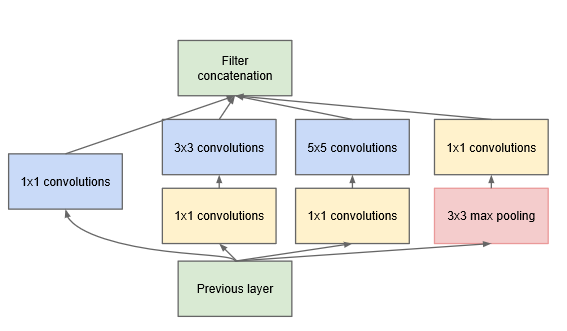
\includegraphics[width=0.55\textwidth]{imgs/inception1.png}
\caption{Inception module. Image source \cite{GoogleNet2015}}\label{fig:inception}
\end{figure}

GoogLeNet consists of nine inception blocks, each containing two layers of inception modules. In total, the network includes 22 layers with parameters, or 27 layers when including the pooling layers.Following G oogleNet (Inception v1), several improved versions have been introduced, such as:
\begin{itemize}[b]
  \item \textbf{Inception v2 and v3}: Introduce batch normalization, factorized convolutions, and other improvements to enhance training and performance.
  \item \textbf{Inception v4 and Inception-ResNet}: Combine Inception modules with residual connections, further improving training efficiency and model accuracy.
\end{itemize}

GoogLeNet (သို့မဟုတ်) Inception v1 ကို ၂၀၁၄ ခုနှစ်တွင်  Google မှ သုတေသနပညာရှင်များက တီထွင်ခဲ့ပါသည်။ အဆိုပါ GoogLeNet ၏ ထူးခြားချက်မှာ အထက်ပါ ပုံတွင် ပြသထားသည့် Inception module ဖြစ်သည်။ 
ပုံရိပ်တစ်ခုတွင် ပါ၀င်သည့် အရေးကြီးသော object ၏ အရွယ်အစားမှာ အမျိုးမျိုး ဖြစ်နေနိုင်ရာ မတူညီသည့် filter size များကို အသုံးပြုခြင်းဖြင့် အမျိုးအစားခွဲခြားရာတွင် အသုံး၀င်သည့် feature များကို ရှာဖွေနိုင်သည်။ GoogLeNet မတိုင်မီ တီထွင်ခဲ့သည့်  Convolutional Neural Network များကို လေ့လာကြည့်မည်ဆိုပါက layer အရေအတွက်  များလာသည်နှင့် အမျှ ပိုမိုကောင်းမွန်သည့် ရလဒ်များကို ရရှိသည်ကို တွေ့ရှိနိုင်သည်။ သို့သော် layer အရေအတွက်  များလာသည်နှင့် အမျှ model ကို Training ပြုလုပ်ရန် အသုံးပြရသည့် ကြာချိန် ပိုလာပြီး computational resource များလည်း ပိုမို လိုအပ်လာသည်။ 

GoogLeNet တွင် ပါ၀င်သည့် Inception module ၏ ထူးခြားချက်မှာ Neural network တစ်ခုတွင်  layer အရေအတွက် ထပ်တိုးရမည့် အစား Layer တစ်ခုထဲတွင် convolution filter size သုံးမျိုးကို အသုံးပြု၍ feature များကို ရှာဖွေခြင်း ဖြစ်သည်။  GoogLeNet တွင် inception block - ၉ ခု ပါ၀င်ပြီး အဆိုပါ  inception block - တစ်ခု၌ ပုံ \ref{fig:inception} တွင် ပြသထားသည့် Inception module နှစ်ခုစီ ပါ၀င်သည်။ ထို့အပြင် convolutional layer များလည်း ပါ၀င်ရာ GoogLeNet ၏ architecture တွင် layer စုစုပေါင်း နှစ်ဆယ့်နှစ်ခု ပါ၀င်သည်။ Pooling Layer များကိုပါ ထည့်သွင်းစဥ်းစားမည်ဆိုပါက layer နှစ်ဆယ့်ခုနစ် ခု ပါ၀င်သည်။ GoogLeNet တွင် fully-connected-layer များအစား average pooling layer နှင့် drop-out layer တို့ကို တွဲ၍ အသုံးပြုထားသည်။ drop-out layer ဆိုသည်မှာ အဆိုပါ layer ရှိ neuron များအနက် ရာခိုင်နှုန်းအချို့ကို ယာယီ ထည့်သွင်း မစဥ်းစားခြင်း ဖြစ်သည်။ GoogLeNet ၏ architecture တွင် rectified linear activation function ကို အသုံးပြုထားသည်။ 

ယနေ့ အချိန်တွင် GoogLeNet ကို အခြေခံသည့် Inception v2 ၊ v3 ၊  v4 နှင့် GoogLeNet နှင့် ResNet တို့ကို ပေါင်းစည်းထားသည့် Inception-ResNet တို့ကို တီထွင်ခဲ့ကြပြီး ဖြစ်သည်။  

\subsection{EfficientNet}

\newpage
\subsection{ConvNeXt}
\newpage


\subsection{Evolution of CNN}

The evolution of Convolutional Neural Networks (CNNs) represents a significant advancement in computer vision, with each architecture improving on previous designs to address specific challenges. This section discussed key architectures such as ConvNet, AlexNet, ResNet, GoogLeNet, EfficientNet, and ConvNext, which form the basis for modern methodologies in object detection and image classification.

YOLO (You Only Live Once) exemplifies the application of these advancements, achieving state-of-the-art performance in real-time object detection. By building on the principles of earlier CNN models, YOLO optimizes for speed and accuracy, revolutionizing various industries and driving innovation in computer vision applications.

ယခု အခန်းတွင် ဆွေးနွေးခဲ့သည့် CNN Architecture အမျိုးမျိုးကို လေ့လာကြည့်ပါက သုတေသန ပညာရှင်များသည် တစ်နှစ်ထက် တစ်နှစ်ထက် ပိုမိုကောင်းမွန်သည့် model များ ထွက်ပေါ်လာရန် ကြိုးစားလာနေသည်ကို တွေ့နိုင်ပါသည်။  ယခု အခန်းတွင် ဆွေးနွေးခဲ့သည့် architecture များအပြင်  CNN architecture အသစ်များသည် အချိန်နှင့် အမျှ ထွက်ပေါ်လာနေသည်။ အဆိုပါ Architecture များ၏ တိုးတက်မှုသည် object detection နှင့် image classification စသည့် computer vision လုပ်ငန်းစဥ် အမျိုးမျိုးကို များစွာ အထောက်အပံ့ဖြစ်သည်။ 

Real time object detection လုပ်ငန်းစဥ်ကို ဆောင်ရွက်ပေးသည့် YOLO (You Only Live Once)  သည် အဆိုပါ ပြောင်းလဲမှုများ၏ တိုးတက်မှု အကျိုးကျေးဇူးကို သိသာထင်ရှားစေသော ဥပမာ တစ်ခုပင် ဖြစ်သည်။ YOLO version များသည် နှစ်စဥ် အသစ်ထွက်ပေါ်လာလျက် ရှိပြီး နောက်ဆုံး ထွက်ပေါ်လာသည့် YOLO v9 သည် accuracy တိုးတက်လာရုံမက computational resources ကို လည်း လျော့ချပေးနိုင်သည်ဟု အဆိုပြုထားကြသည်။ 


\newpage
\section{Datasets for Computer Vision Tasks}
In the field of computer vision, several datasets \cite{web:cvDatasets} have become essential benchmarks for various tasks such as image classification, object detection, and segmentation. The most commonly used datasets are listed below:
\begin{itemize}[b] 
\item \textbf{ImageNet}:  ImageNet \cite{web:ILSVRC} is one of the largest image datasets available, containing over 14 million labeled images across 20,000 categories. It is primarily used for image classification and object recognition tasks. The ImageNet Large Scale Visual Recognition Challenge (ILSVRC) has driven significant advancements in the field of deep learning and computer vision. Models like AlexNet, VGG, ResNet, and GoogLeNet were benchmarked on this dataset. Some sample images from ImageNet are shown in Figure \ref{fig:imgNet}.
    \item \textbf{Pascal VOC}: PASCAL Visual Object Classification (PASCAL VOC) 2007 and 2012 \cite{web:Pascal} is a familiar and widely used dataset for object detection object detection, classification, and segmentation. It includes a series of yearly challenges with datasets that feature annotated objects across 20 different categories.
    \item \textbf{COCO}: The common Objects in COntext (COCO) dataset \cite{web:CoCo} was developed by Microsoft team. It is a large-scale dataset for object detection, segmentation, and captioning. It contains over 330,000 images with more than 1.5 million object instances, labeled with 80 object categories.
    \item \textbf{Open Images Dataset}: Open Images \cite{web:OpenImage} is a large-scale dataset for object detection, image classification, and visual relationship detection. The dataset contains about 9.2 million labeled and unified ground-truth images and segmentation masks. This database has about 600 object classes with almost 16 million bounding boxes. It is considered one of the largest databases for object localization.
\end{itemize}

\vspace{0.5em}
\begin{figure}[h]%
\centering
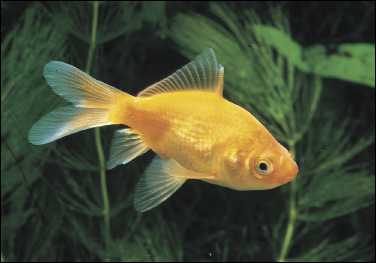
\includegraphics[width=0.25\textwidth]{imgs/imgnet_1.jpeg}
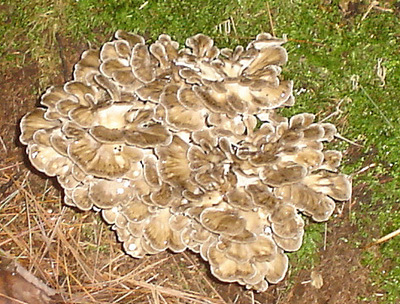
\includegraphics[width=0.25\textwidth]{imgs/imgnet_2.jpeg}
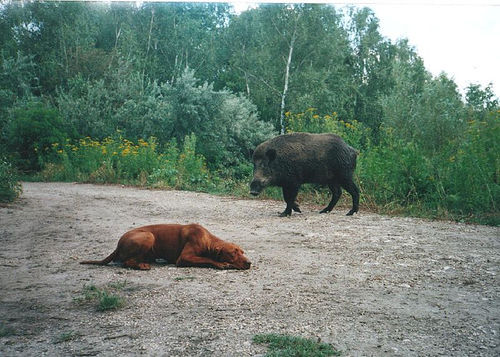
\includegraphics[width=0.25\textwidth]{imgs/imgnet_3.jpeg}
\caption{Sample images from ImageNet\cite{web:ILSVRC}}\label{fig:imgNet}
\end{figure}

Computer vision ဘာသာရပ်တွင် ယုံကြည်စိတ်ချရသော dataset များသည် AI model များ တီထွင်ဖန်တီးနိုင်ခြင်း၏ အသက်ဖြစ်သည်။ သို့သော် အဆိုပါ datasetများကို ဖန်တီးတည်ဆောက်ရန်မှာ မလွယ်ကူပါ။ Computer vision ဘာသာရပ်တွင် အသုံးများသည့် datasetများမှာ အောက်ပါအတိုင်း ဖြစ်သည်။ 

\begin{itemize}[b] 
\item \textbf{ImageNet}:  ImageNet \cite{web:ILSVRC} တွင် ကား၊ ပရိဘောဂ၊ အ၀တ်အစား၊ အစားအသောက် စသည်ဖြင့် အမျိုးအစားပေါင်း ၂ သောင်း၏ image စုစုပေါင်း တစ်ဆယ့် လေးသန်းကျော်ပါ၀င်သည်။ Image classification နှင့် object recognition လုပ်ငန်းစဥ်များ၊ပြိုင်ပွဲများတွင် အများဆုံး အသုံးပြုခဲ့ကြသည့် dataset လည်းဖြစ်သည်။ ImageNet Large Scale Visual Recognition Challenge (ILSVRC)  ပြိုင်ပွဲကို ၂၀၁၀ မှ ၂၀၁၇ အထိ နှစ်စဥ် ကျင်းပခဲ့ကြပြီး ILSVRC တွင် အမျိုးအစားပေါင်း တစ်ထောင် ၏ ဓါတ်ပုံ တစ်ဆယ့်နှစ်သန်းကျော်ပါ၀င်သည့်  dataset ကို အသုံးပြုယှဥ်ပြိုင်ခဲ့ကြသည်။ အထက်တွင် ဆွေးနွေးခဲ့သည့် AlexNet, VGG, ResNet, နှင့် GoogLeNet တို့တွင် ၄င်းတို့၏ စွမ်းဆောင်ရည်ကို တိုင်းတာနိုင်ရန် ဤ dataset ကို အသုံးပြုခဲ့ကြသည်။ 
    \item \textbf{Pascal VOC}: PASCAL Visual Object Classification (PASCAL VOC) 2007 and 2012 \cite{web:Pascal} သည်လည်း လူသုံးများသည့် အခြား dataset တစ်ခု ဖြစ်သည်။ ဤ datasetကို အသုံးပြု၍ နှစ်စဥ်ပြိုင်ပွဲ ပြုလုပ်လေ့ရှိပြီး ကား၊ လေယာဥ်ပျံ၊ စက်ဘီး၊ ငှက်၊ လှေစသည်ဖြင့် အမျိုးအစားပေါင်း ၂၀ ကျော်၏  image စုစုပေါင်း ၃ ထောင်ကျော်ပါ၀င်သည်။ 
    \item \textbf{COCO}: Microsoft အဖွဲ့မှ ထုတ်လုပ်သည့် COCO) dataset \cite{web:CoCo}တွင် မတူညီသည့် အမျိုးအစားပေါင်း ၈၀ အတွက်   image စုစုပေါင်း သုံးသိန်း သုံးသောင်းကျော် ပါ၀င်သည်။ 
    \item \textbf{Open Images Dataset}: Open Images \cite{web:OpenImage} သည် နောက်ဆုံး ထွက်ထားသည့် dataset ဖြစ်ပြီး image စုစုပေါင်း ကိုးသန်း နှစ်သိန်းကျော်ပါ၀င်သည်။ မတူညီသည့် အမျိုးအစား - ၆၀၀ ကျော်ပါ၀င်ပြီး image အတွင်ရှိ object ၏ နေရာကို အတိအကျပေးထားသည့် bounding box ၁၆ သန်းပါ၀င်သည်။ 
\end{itemize}

\newpage
\section{Case Study: Image Classification}

This section presents two distinct case studies showcasing the application of deep learning in image classification. The first project explores object classification using various CNN architectures discussed in section \ref{sec:vCNN}, while the second delves into handwritten digit recognition. Both projects aim to leverage deep learning techniques to solve practical image classification tasks.

ဤအခန်းတွင် လက်တွေ့ သင်ခန်းစာများအဖြစ် project - နှစ်ခုကို တင်ပြထားသည်။ ပထမ project မှာ အထက်၌ တင်ပြထားခဲ့သည့် CNN architecture များကို အသုံးပြု၍ image များကို အမျိုးအစား ခွဲခြင်းခြင်းဖြစ်ပြီး ဒုတိယ project တွင်မူ လက်ရေးဖြင့် ရေးထားသော သင်္ချာ ကိန်းဂဏန်းများကို အလိုအလျောက်ခွဲခြားပေးနိုင်မည့် deep learning architecture တစ်ခု တည်ဆောက်ရန် ဖြစ်သည်။ 

\subsection{Case Study-1: Object Classification using different CNN architectures}

In this project, AI-generated images are classified using five  state-of-the-art Convolutional Neural Network (CNN) models implemented with the Python `keras` library. The models used are `\texttt{ResNet50}`, `\texttt{VGG16}`, `\texttt{InceptionV3}`, `\texttt{ConvNeXtTiny}`, and `\texttt{EfficientNetB7}`. The goal is to load an image, pass it through each of these models, and obtain the top prediction for the image as shown in Figure \ref{fig:p1R}. 

This project consists of two Python scripts: one for defining the CNN models (`\texttt{cnn\_models.py}`) and one main script (`\texttt{main.py}`) for classifying an image.

\vspace{0.5em}
\begin{figure}[h]%
\centering 
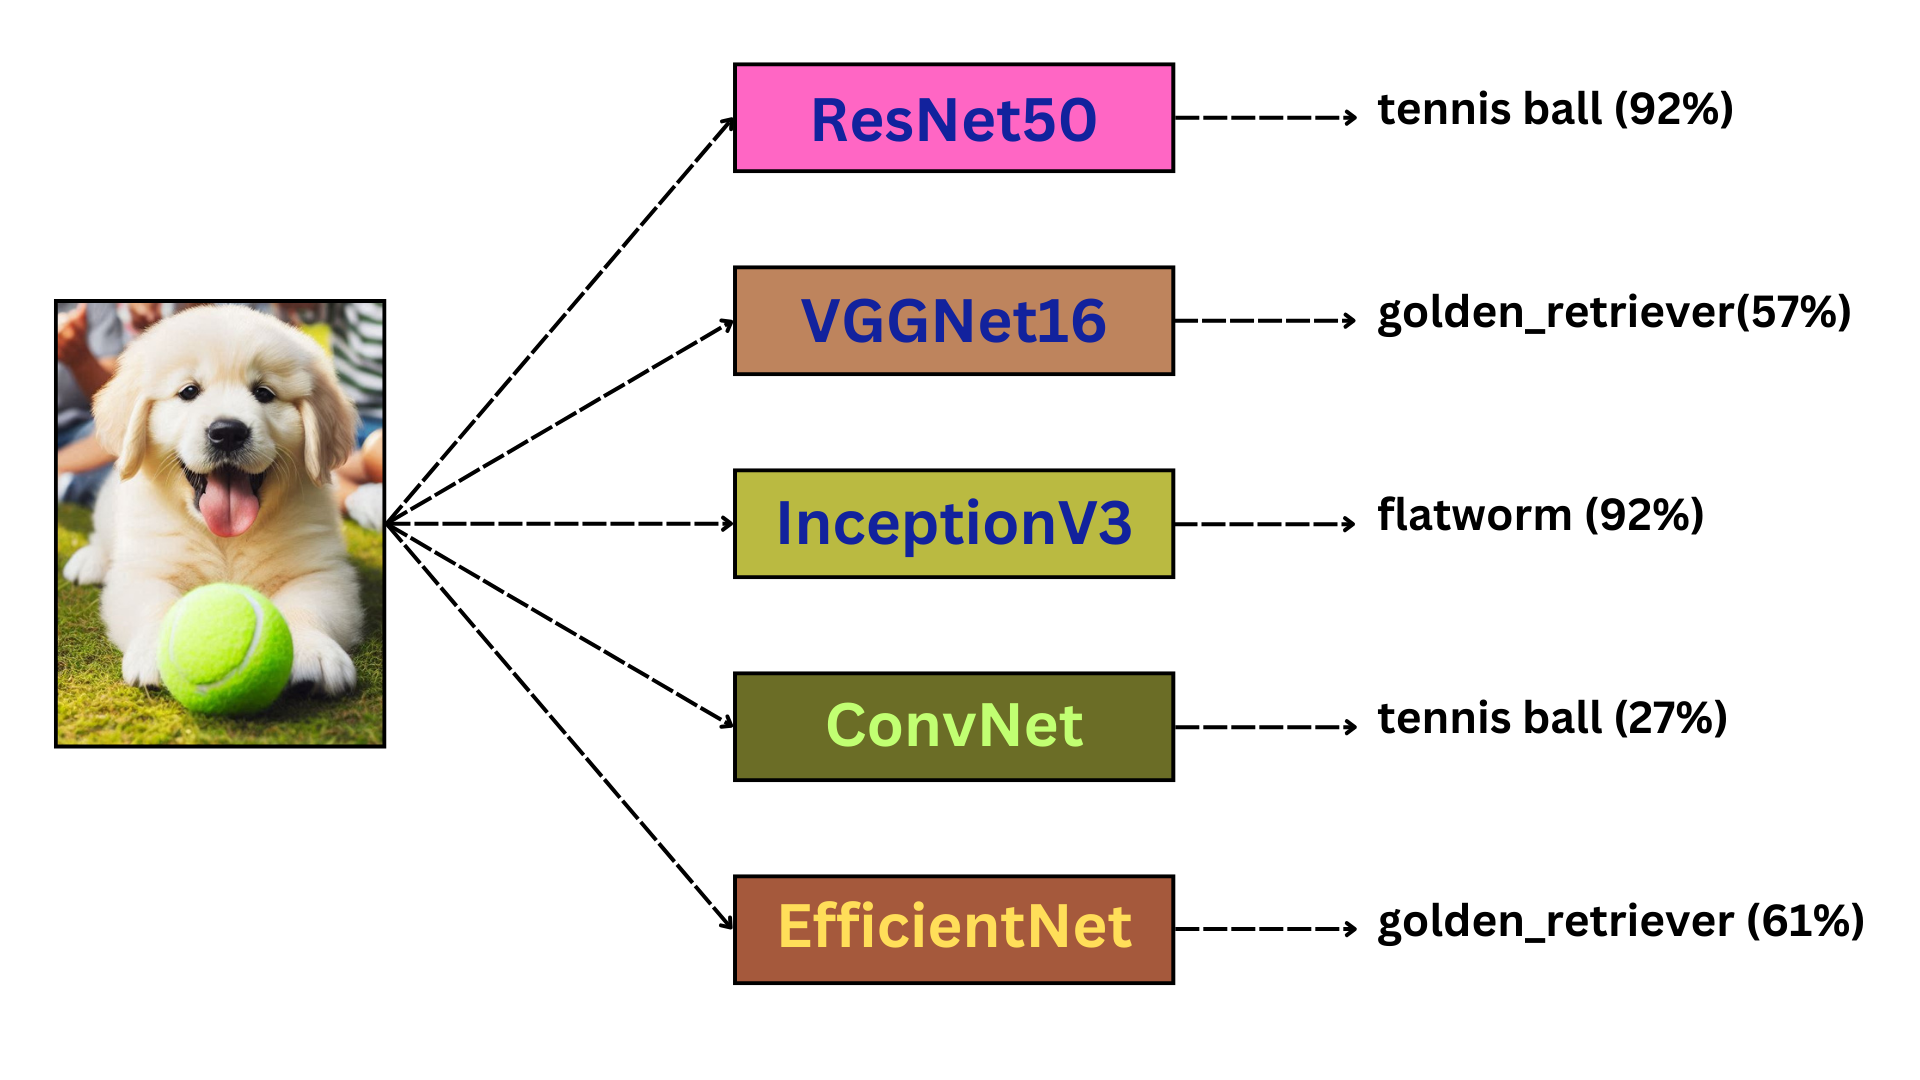
\includegraphics[width=0.8\textwidth]{imgs/p1_result.png}
\caption{Prediction of Objects by 5 different state-of-the-art CNN architectures}\label{fig:p1R}
\end{figure}

ပထမ project မှာ အခန်း \ref{sec:vCNN} တွင် ဆွေးနွေးခဲ့သည့် CNN architecture များအနက် - ငါးခုကို အသုံးပြု၍ AI ဖြင့် ဖန်တီးယူထားသည့် ပုံရိပ်များကို အမျိုးအစား ခွဲခြားခြင်း ဖြစ်သည်။ ယခု project တွင် အသုံးပြုမည့်  CNN architecture များမှာ  `\texttt{ResNet50}`, `\texttt{VGG16}`, `\texttt{InceptionV3}`, `\texttt{ConvNeXtTiny}`, နှင့် `\texttt{EfficientNetB7}`တို့ ဖြစ်ကြသည်။ 

ယခု  project တွင် (`\texttt{cnn\_models.py}`) နှင့် (`\texttt{main.py}`) ပါ၀င်သည်။ ပထမ  script  (`\texttt{cnn\_models.py}`) ၍ Python `keras` library တွင် pre-trained ပြုလုပ်ထားပြီး ဖြစ်သည့် CNN model များကို ခေါ်ယူ အသုံးပြုရန် ရေးထားသည့် class ဖြစ်သည်။ အဆိုပါ class တွင် ခေါ်ယူ အသုံးပြုမည့် CNN architecture များ၏ အမည်ကို သတ်မှတ်သည့် function ၊ CNN architecture များကို initialize လုပ်သည့် function များနှင့် input image ကို classify လုပ်မည့် function များ ပါ၀င်သည်။ 

ဒုတိယ script (`\texttt{main.py}`)  သည် (`\texttt{cnn\_models.py}`) ကို အသုံးပြု၍ ပုံရိပ်တစ်ခုကို ခွဲခြားပေးသည်။ 

\newpage
\subsubsection{Python Implementation}

\begin{itemize}[b]
\item{ \texttt{`cnn\_models.py`}}: This script defines a class, \texttt{`cnnModels`}, which provides an interface to load and use the pre-trained CNN models. The class includes methods for initializing models, retrieving models by name, and classifying images.

\item{\texttt{ `main.ipynb`}}: This script demonstrates how to use the `cnnModels` class to classify an image.
\end{itemize}

\begin{solution}
\begin{lstlisting}
    class cnnModels:
        def __init__(self):
            self.models = {'ResNet50': self.resnet(), 'VGGNet16': self.vggnet(), 
                           'InceptionV3': self.inception(), 'ConvNet': self.convnet(), 
                           'EfficientNet': self.efficientnet()}
    
        def resnet(self):       
            model = ResNet50(weights='imagenet')
            return model
        
        def vggnet(self):
            model = keras.applications.VGG16(weights='imagenet')
            return model
        
        def inception(self):
            model = keras.applications.InceptionV3(weights='imagenet')
            return model
        
        def convnet(self):
            model = keras.applications.ConvNeXtTiny(weights='imagenet')
            return model       
        
        def efficientnet(self):
            model = keras.applications.EfficientNetB7(weights='imagenet')
            return model
    
        def get_model(self, name):
            if name in self.models:
                return self.models[name]
            else:
                raise ValueError(f"Model '{name}' does not exist.")            
            
        def classify_image(self, name, img):
            model = self.get_model(name)      
            
            img = img.resize((model.input_shape[1], model.input_shape[2]))  
            x = img_to_array(img)
            x = np.expand_dims(x, axis=0)
            x = preprocess_input(x)
            
            preds = model.predict(x)
            return decode_predictions(preds, top=1)

\end{lstlisting}  
\end{solution}

\begin{solution}
\begin{lstlisting}
    from cnn_models import cnnModels
    from keras.preprocessing.image import load_img
    
    img_path = './imgs/dog.jpeg'
    img = load_img(img_path)
    
    model = cnnModels()    
    preds1 = model.classify_image('ResNet50', img)
    
    for pred in preds1:
        print(f"{pred[1]}: {pred[2]}, {pred[3]}")
\end{lstlisting}

\end{solution}
\vspace{0.5em}
\begin{figure}[h]%
\centering 
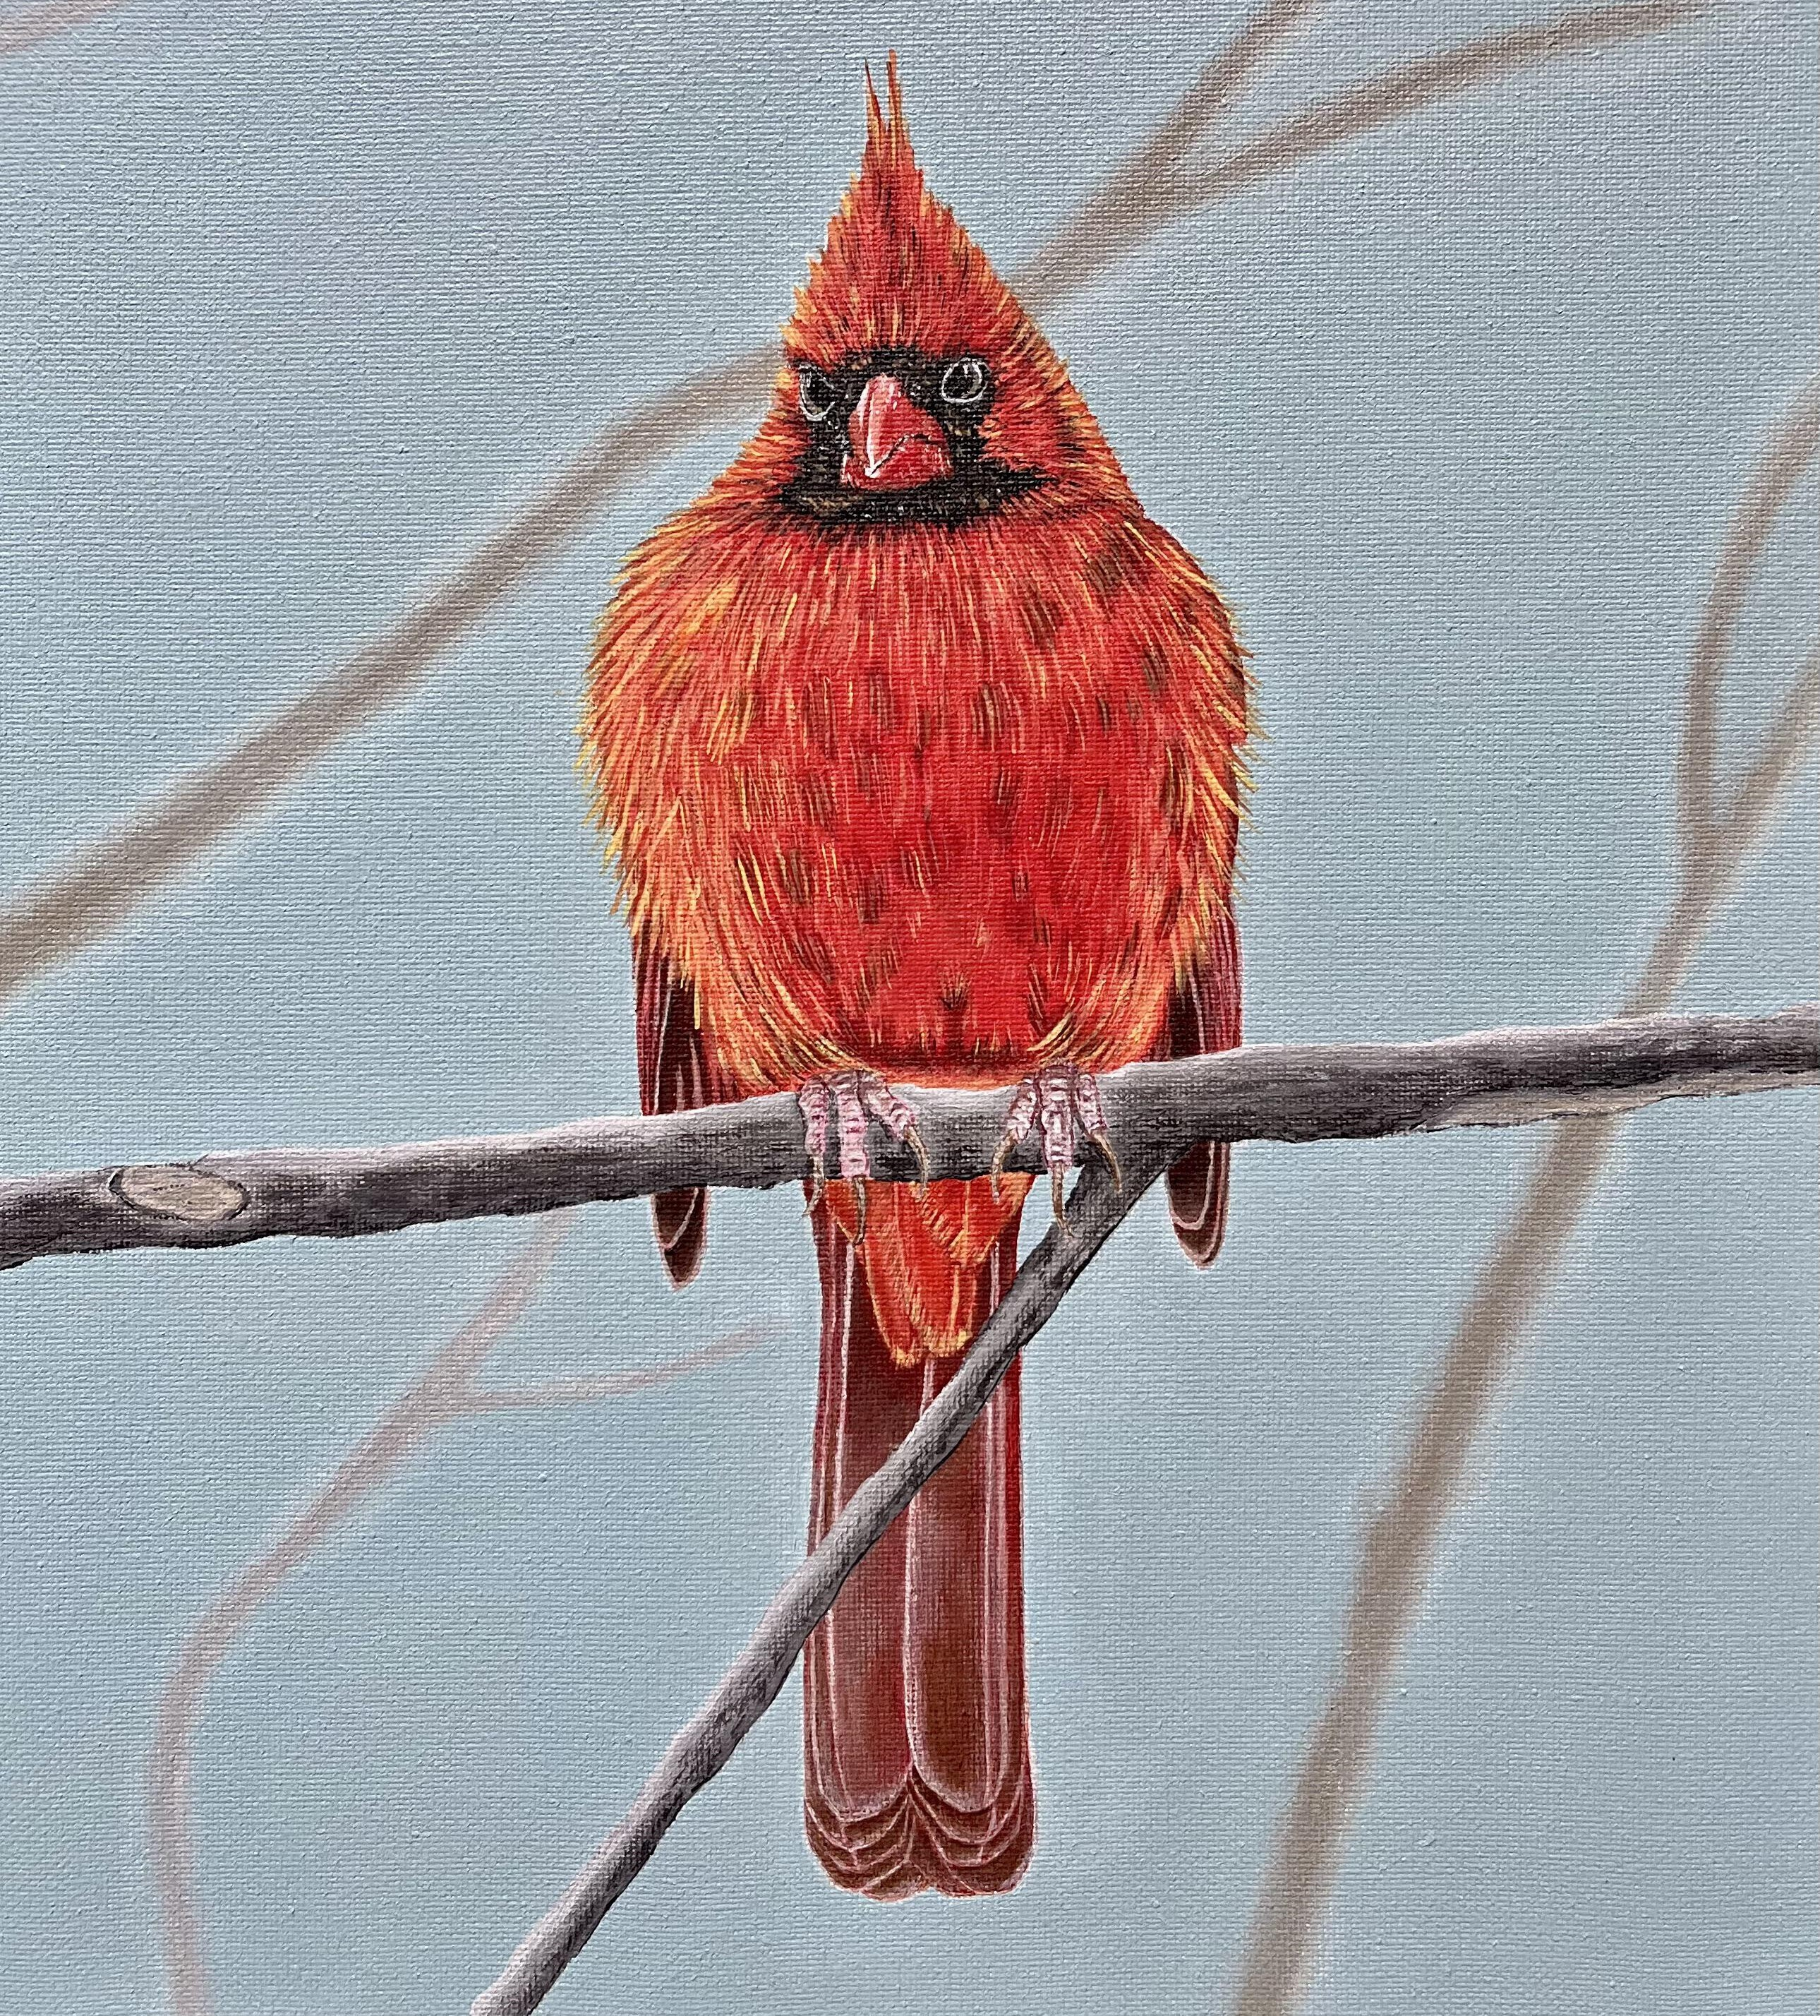
\includegraphics[width=0.23\textwidth]{imgs/bird.jpg}
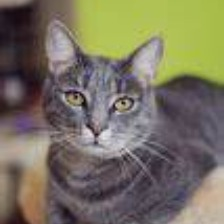
\includegraphics[width=0.24\textwidth]{imgs/cat.jpg}
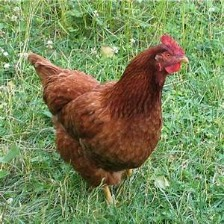
\includegraphics[width=0.24\textwidth]{imgs/chicken.jpg}
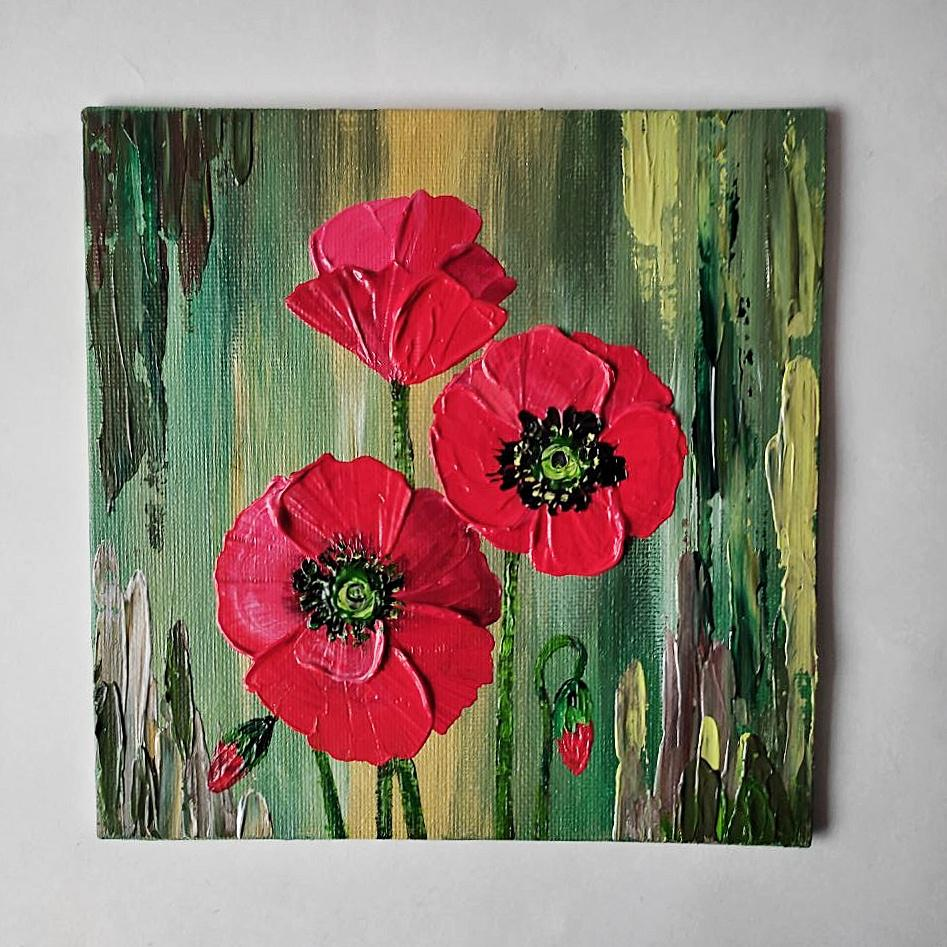
\includegraphics[width=0.24\textwidth]{imgs/flower.jpg}

\includegraphics[width=0.24\textwidth]{imgs/bird.jpeg}

\includegraphics[width=0.24\textwidth]{imgs/cat.jpeg}
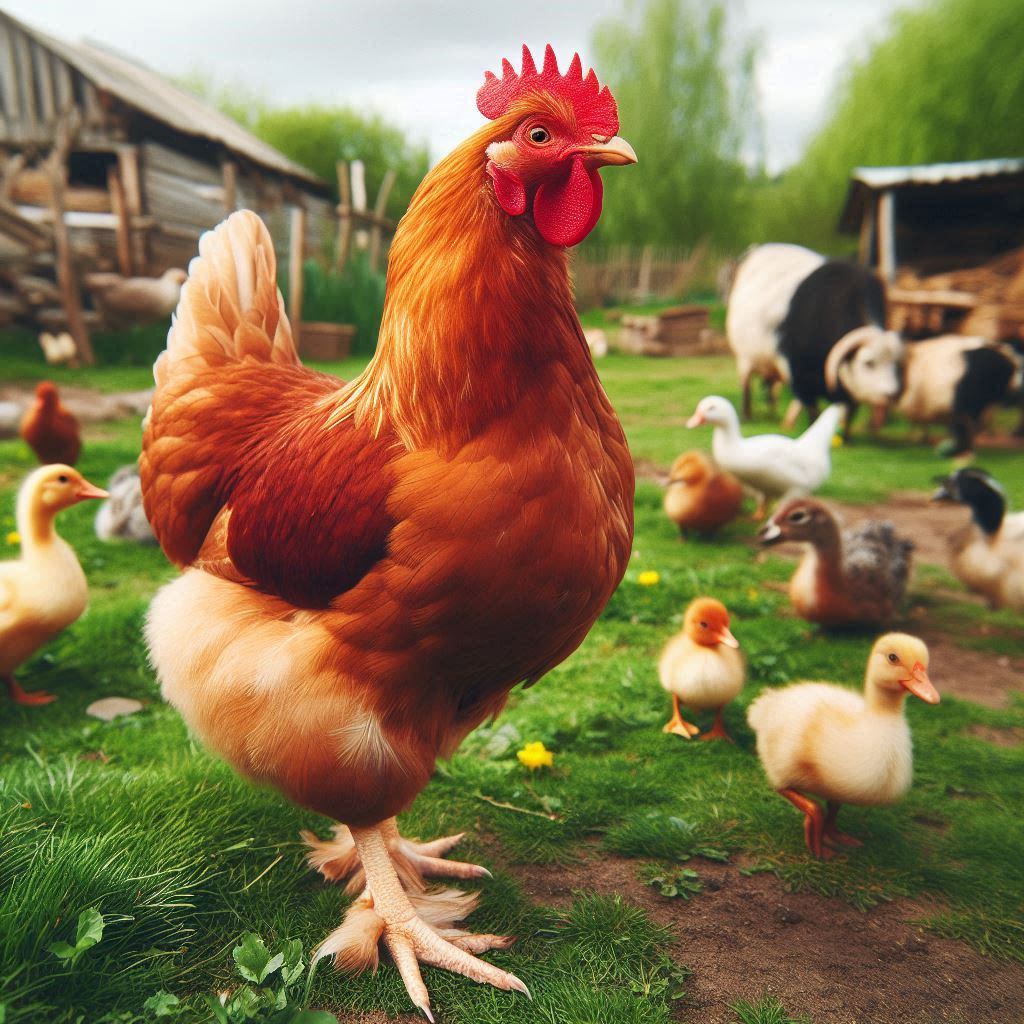
\includegraphics[width=0.24\textwidth]{imgs/chicken.jpeg}

\includegraphics[width=0.24\textwidth]{imgs/rose.jpeg}
\caption{Sample Images. The first row displays real images collected from the internet, whereas the second row shows synthetic images generated using AI.}\label{fig:p1R}
\end{figure}
\subsubsection{Dataset}
In this project, a small dataset comprising 20 images is utilized. This dataset includes 10 real images collected from the internet and 10 synthetic images generated using Microsoft Image Generator \cite{web:MSimgCreator}. The sizes of the real images are random, while the synthetic images have a fixed dimension of 1024 x 1024 pixels. These images are pre-processed before being fed into the cnnModel module explained above.

ဤ project တွင် real image တစ်ဆယ်ခုနှင့် AI အသုံးပြု၍ ဖန်တီထားသည့် ပုံရိပ် ဆယ်ခုတို့ကို အသုံးပြု၍ image classification ပြုလုပ်ပြသွားမည်ဖြစ်သည်။ real image များမှာ အင်တာနက်မှ ရယူထားခြင်းဖြစ်ရာ ၄င်းတို့၏ image size မှာ 214 x 214 မှ 2567x 2586 အထိ အမျိုးမျိုး ပါ၀င်သည်။ AI အသုံးပြု၍ ဖန်တီထားသည့် ပုံရိပ်များ၏ image size မှာ 1024 x 1024 ဖြစ်သည်။ အထက်တွင် ဖော်ပြထားသည့် cnnModel module ကို အသုံးပြု၍ image များကို အမျိုးအစားမခွဲခြားမီ သက်ဆိုင်ရာ CNN model များမှ လိုအပ်သည့် အရွယ်အစားကို ရအောင် ညှိပေးရမည် ဖြစ်သည်။ ဥပမာ  VGGNet နှင့် ResNet Model များအတွက် input image ၏ အရွယ်အစားမှာ 224 x 224 ဖြစ်သည်။ 

\subsubsection{Results and Discussion}

\newpage
\subsection{Case Study-2: Handwritten Digit Recognition}
Handwritten digit recognition is a classic problem in computer vision and machine learning, involving training a model to classify handwritten digits (0-9) from images. While numerous solutions exist for English digit recognition, there's a limited resources for recognizing digits in languages like Myanmar. The objective of this project is to bridge this gap by developing a machine learning model capable of recognizing handwritten digits in the Myanmar language. This task holds significant importance for various applications, including digitization efforts, character recognition systems, and automation technologies. However, Myanmar script presents unique challenges, such as variations in writing styles, stroke thickness, and complex shapes, making digit recognition a non-trivial task. Therefore, the development of an efficient architecture tailored to address these challenges is crucial for the advancement of the Myanmar community in the journey of technology.

လက်ရေးဖြင့် ရေးထားသော နံပါတ်များကို ကွန်ပြူတာမှ နားလည်စေရန် လေ့ကျင့်ပေးသည့် လုပ်ငန်းစဥ်သည် computer vision လောကတွင် အရေးကြီးသည့် ပြဿနာတစ်ခုဖြစ်ပြီး Method ပေါင်းများစွာ တီထွင်ခဲ့ကြပြီး ဖြစ်သည်။ ဤ လုပ်ငန်းစဥ်သည် လက်ရေးဖြင့် ရေးထားသော စာရွက်စာတမ်းများကို ကွန်ပြူတာဖြင့် သိမ်းဆည်းနိုင်ရန် အတွက် အရေးကြီးသော အဆင့်တစ်ခု ဖြစ်သည်။ အင်္ဂလိပ် ဘာသာစကားဖြင့် ရေးသားထားသော နံပါတ်များကို ကွန်ပြူတာမှ နားလည်စေရန် လေ့ကျင့်ပေးထားသော AI tool များစွာ ရှိသော်လည်း မြန်မာ ဘာသာဖြင့် ရေးသားထားသော ဂဏန်းများအတွက် လေ့ကျင့်ပေးထားသော Programme သည် အကန့်အသတ်ဖြင့်သာ ရှိနေသေးသည်။ မြန်မာ နံပါတ်များသည် တမူကွဲပြားသည့် ရေးဟန် ရှိရာ မြန်မာ ဘာသာစကားအတွက် သီးသန့် ရည်ရွယ်သည့် Method များထွက်ပေါ်လာရန် လိုအပ်သည်။ ယခု Project တွင် လက်ရေးဖြင့်ရေးသားထားသည့် မြန်မာ နံပါတ်များကို နားလည်နိုင်ရန်အတွက် CNN ကို အခြေခံသည့် deep learning model တစ်ခု တည်ဆောက်သွားမည် ဖြစ်သည်။ 

\subsubsection{Dataset}
In handwritten digit recognition, the MNIST dataset \cite{web:mnist} is a commonly used benchmark, featuring 28x28 grayscale images of English handwritten digits. However, the MNIST dataset is limited to digits written in English. In this project, we utilized a dataset from \cite{web:MMdataset}, containing 2,200 images of Myanmar handwritten digits, with each digit represented by 220 images. Some sample images are shown in Figure \ref{fig:p2MMdigits}. Seventy percent of the images (1,540) were used for training, while the remaining 30 percent (660) were reserved for testing.

လက်ရေးဖြင့် ရေးထားသည့် နံပါတ်များနှင့် ပတ်သတ်သည့် Project များ ပြုလုပ်ရာတွင် ၁၉၉၈ ခုနှစ်က သုတေသနပညာရှင် Yann LeCun နှင့် အဖွဲ့ ထုတ်ခဲ့သည့်  MNIST dataset ကို အများဆုံး အသုံးပြုကြသည်။ အဆိုပါ dataset သည်  အင်္ဂလိပ် ဘာသာစကားဖြင့် ရေးသားထားသော နံပါတ်များအတွက် အကောင်းဆုံး ဖြစ်သော်လည်း မြန်မာဘာသာဖြင့် ရေးထားသည့် နံပါတ်များ မပါ၀င်ပါ။ သို့ဖြစ်ရာ ဤ Project တွင် မြန်မာ လူငယ်များ စုစည်းထားသည့် လက်ရေးဖြင့်ရေးထားသည့် မြန်မာ နံပါတ်များပါ၀င်သည့် dataset ကို အသုံးပြုခဲ့သည်။ အဆိုပါ dataset တွင် နံပါတ် တစ်ခုစီအတွက် image နှစ်ရာ့ နှစ်ဆယ်စီ ပါ၀င်ရာ image စုစုပေါင်း နှစ်ထောင့်နှစ်ရာ ပါ၀င်သည်။ ထိုအထဲမှ ခုနစ်ဆယ် ရာခိုင်နှုန်းကို training အတွက် အသုံးပြုခဲ့ပြီး ကျန် သုံးဆယ် ရာခိုင်နှုန်းကို testing အတွက် အသုံးပြုထားသည်။ ဤ dataset တွင် ပါ၀င်သည့် နမူနာ image အချို့ကို အောက်တွင် ပြသထားသည်။ 

\vspace{0.5em}
\begin{figure}[h]%
\centering 
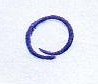
\includegraphics[width=0.15\textwidth]{imgs/0.jpg}

\includegraphics[width=0.15\textwidth]{imgs/1.jpg}

\includegraphics[width=0.15\textwidth]{imgs/2.jpg}

\includegraphics[width=0.15\textwidth]{imgs/3.jpg}
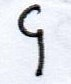
\includegraphics[width=0.12\textwidth]{imgs/4.jpg}
\caption{Sample Images of Myanmar handwritten digits.}\label{fig:p2MMdigits}
\end{figure}

\subsubsection{Data Preprocessing}
The images of handwritten digits are initially provided as 310x219 gray-scale matrices. Since the region of interest (the handwritten digit) is relatively small, approximately 80x80 pixels and centered, the first step in data preprocessing is to \texttt{crop} the image by removing 50 pixels from the left and right, and 20 pixels from the top and bottom. This results in an image size of 270x179 pixels. 

Next, to prepare the images for input into the proposed deep learning architecture, the cropped images are \texttt{resized} to 64x64 pixels. This resizing step ensures uniformity in the input data dimensions, which is crucial for effective processing by the neural network. By reducing the image dimensions, the model can focus on the essential features of the handwritten digits, improving both efficiency and performance in training and evaluation.

Furthermore, an additional dimension is needed for the Convolutional Neural Network (CNN) model. Therefore, the resized images are \texttt{reshaped} to have a shape of $(Nx 64x 64x 1)$, where N is the number of images. This reshaping ensures that the data is in the correct format, with the final dimension representing the single channel of the gray-scale images.

ဤ Project အတွက် အသုံးပြုသည့် dataset ရှိ  image ၏ အရွယ်အစားမှာ 310x219 ဖြစ်ပြီး gray-scale image များဖြစ်ကြသည်။ သို့သော် image တွင် ပါ၀င်သော နံပါတ်များသည် image ၏ အလယ်လောက် တွင် ရှိပြီး နံပါတ်သည် image ၏ အရွယ်အစား နှင့်နှိုင်းယှဥ်လျှင် သေးငယ်သည်။ သို့ဖြစ်ရာ ပထမ ဦးစွာ ပေးထားသည့် gray-scale image များ၏ အနားသတ်ကို ဖြတ်ထုတ်ခြင်းဖြင့် image အရွယ်အစားများ သေးငယ်အောင် ပြုလုပ်သည်။ image ၏ အပေါ် ၊ အောက်မှ pixel နှစ်ဆယ် စီနှင့် ဘေး - ဘယ်၊ ညာမှ 20 pixel ငါးဆယ်ဆီကို ဖြတ်ထုတ်လိုက်ရာ crop လုပ်ပြီးသွားချိန်တွင် image ၏ အရွယ်အစားမှာ 270x179 pixel သာ ရှိတော့သည်။ 

ဒုတိယ အဆင့်တွင် cropped လုပ်ထားသည့် image များကို 64x64 pixel သာ ရှိသည့် အရွယ်အစား သေးငယ်သော image များ ဖြစ်အောင် ချုံ့ခြင်း ဖြစ်သည်။ Deep Learning model များ တည်ဆောက်ရာတွင် ပေးချက် အဖြစ်ပေးမည့် image များသည် အရွယ်အစားတစ်ခုထဲ ဖြစ်နေရန် လိုအပ်ပါသည်။ ထို့နောက် အဆိုပါ image များကို တည်ဆောက်ထားသည့် Convolutional Neural Network (CNN) model ၏ input နှင့် format ဖြစ်သည့် (64x 64x 1) နှင့် ကိုက်ညီစေရန် reshape ပြန်လုပ်ပေးသည်။ Data Preprocessing ပြုလုပ်ပြီးသည့်နောက်တွင် Input Matrix ၏ အရွယ်အစားသည် (N x 64 x 64 x 1) ရှိသည်။ 

\subsubsection{Proposed Architecture}
The proposed architecture follows a common pattern for CNNs used in image classification tasks. It starts with convolutional layers to extract features, followed by flattening and fully connected layers for classification.

\vspace{0.5em}
\begin{figure}[h]%
\centering 
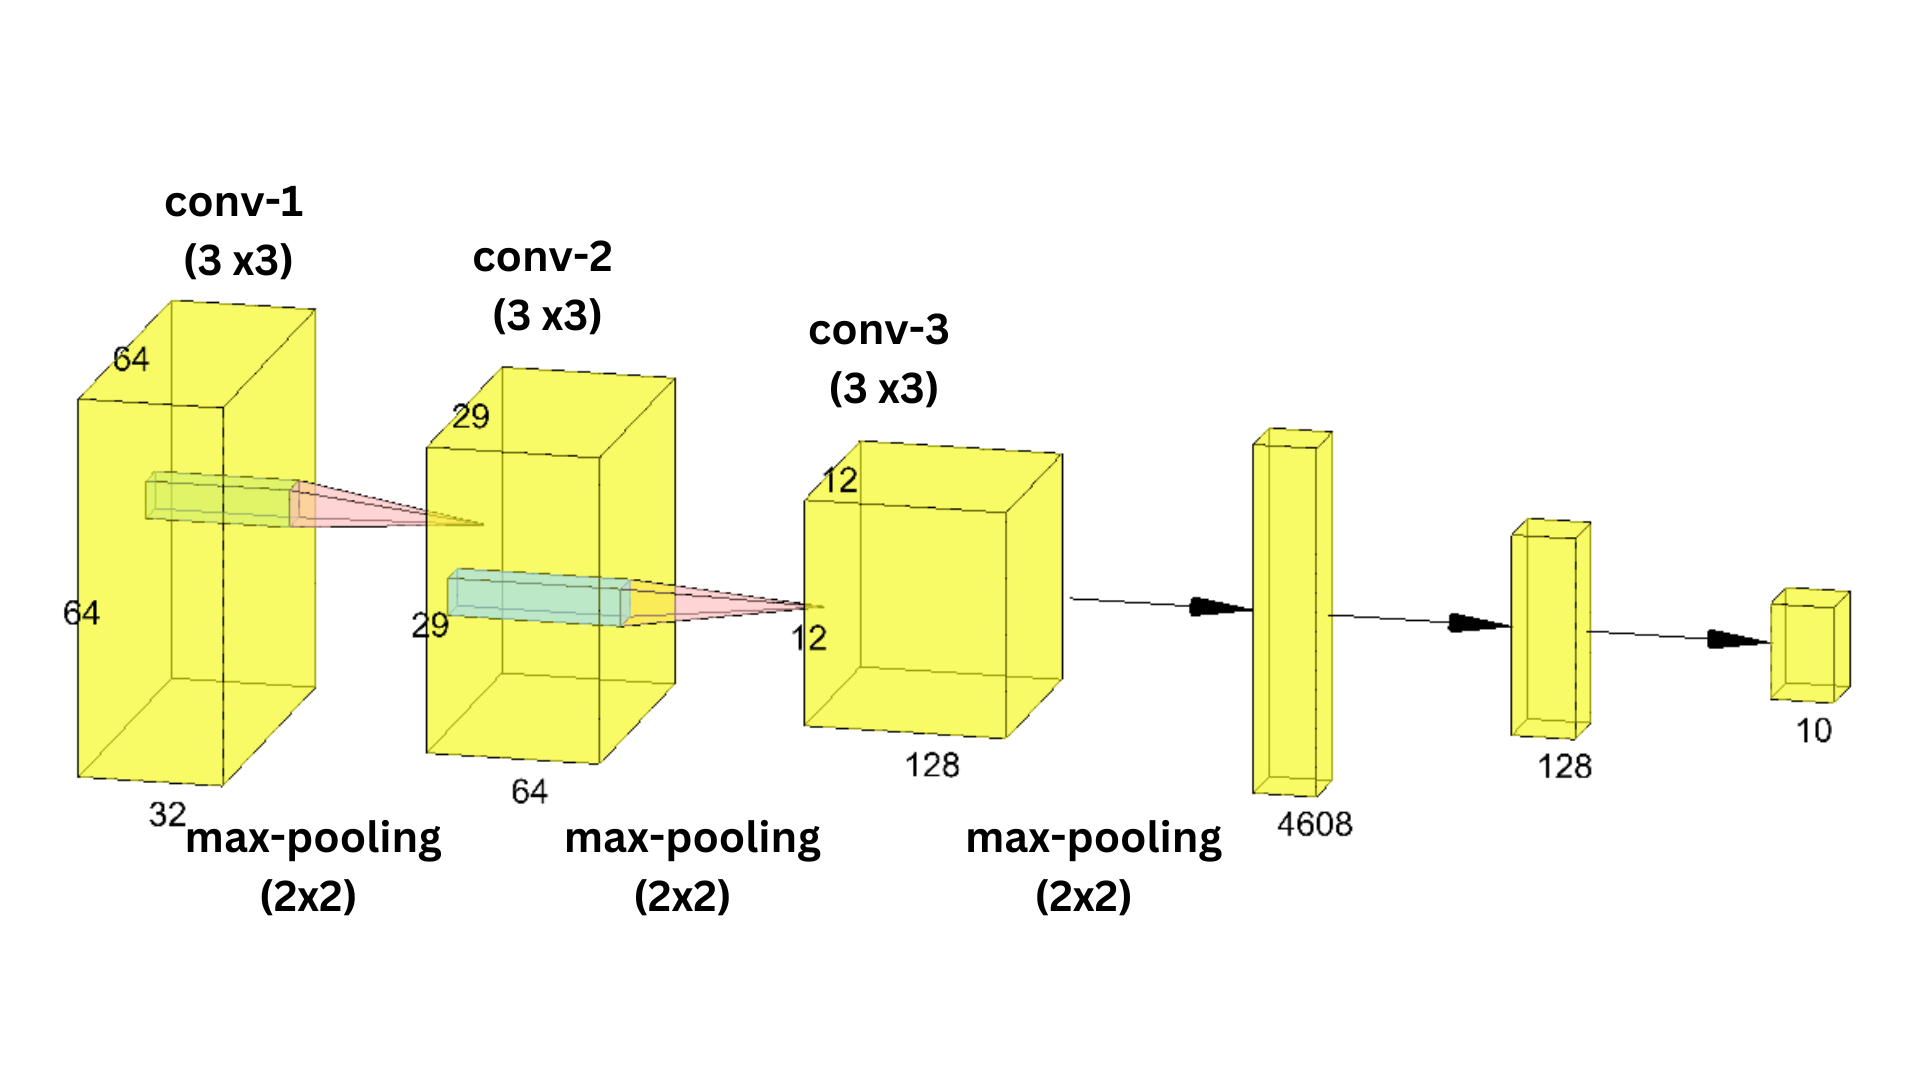
\includegraphics[width=0.75\textwidth]{imgs/p2ThidaNet.png}
\caption{Proposed Architecture for Myanmar handwritten digits Recognition.}\label{fig:p2Net}
\end{figure}

\begin{enumerate}
    \item \textbf{Input Layer}:
        \begin{itemize}
            \item The input layer is defined with the shape of $(64, 64, 1)$, accepts grayscale images of size $64 \times 64$ pixels.
        \end{itemize}
    
    \item \textbf{Convolutional Layers}:
        \begin{itemize}
            \item Three convolutional layers are added successively.
            \item The first layer has $32$ filters with a kernel size of $(3, 3)$ and ReLU activation function.
            \item The second layer has $64$ filters with the same kernel size and activation function.
            \item The third layer has $128$ filters with the same kernel size and activation function.
            \item After each convolutional layer, a max-pooling layer is applied with a pool size of $(2, 2)$, which helps in downsampling and extracting important features.
        \end{itemize}
    
    \item \textbf{Flatten Layer}:
        \begin{itemize}
            \item The output from the convolutional layers is flattened into a $1$D tensor, which will be fed into the fully connected layers.
        \end{itemize}
    
    \item \textbf{Fully Connected Layers}:
        \begin{itemize}
            \item There is a single fully connected hidden layer with $128$ neurons and ReLU activation function.
        \end{itemize}
    
    \item \textbf{Output Layer}:
        \begin{itemize}
            \item The output layer consists of $10$ neurons, representing the 10 classes of digits, with a softmax activation function. Softmax ensures that the output values are probabilities, summing up to $1$, which makes it suitable for multi-class classification tasks.
        \end{itemize}
    
    \item \textbf{Model Compilation}:
        \begin{itemize}
            \item The model is compiled using the Adam optimizer, categorical cross-entropy loss function (suitable for multi-class classification), and accuracy as the metric to monitor during training.
        \end{itemize}
\end{enumerate}

The proposed architecture has trainable parameters of 683,914 (2.61 MB) and the details breakdowns of the parameters for each layer is given below. 

Proposed လုပ်ထားသည့် Architecture တွင် feature များ ရယူရန်အတွက် convolutional နှင့် max-pooling layer များကို အသုံးပြုထားသည်။ convolutional layer သုံးခုတွင် 3x3 filter နှင့်  ReLU activation function ကို သုံးထားပြီး max-pooling layer တွင် 2x2 filter ကို အသုံးပြုသည်။ ထို့နောက် convolutional layer များမှ ရရှိလာသည့် output ကို flattened ပြုလုပ်ပြီး classification လုပ်ရန်အတွက် fully connected layer နှစ်ခုကို အသုံးပြုထားသည်။ နောက်ဆုံး output layer တွင် neuron (unit) ဆယ်ခုပါ၀င်ပြီး softmax activation function ကို အသုံးပြုထားသည်။ အဆိုပါ softmax function မှ  output ဆယ်ခု သည် မြန်မာ နံပါတ်တစ်ခုချင်းစီ၏ ဖြစ်နိုင်ချေ ရာခိုင်နှုန်းကို ညွှန်းဆိုသည်။ model ကို Compilation ပြုလုပ်ရန် Adam optimizer ကို အသုံးပြုထားပြီး accuracy တန်ဖိုးကို maximize လုပ်နိုင်သည့် parameter များကို ရှာဖွေစေခြင်းဖြစ်သည်။ 

ယခု model တွင် training ပြုလုပ်စဥ် ရှာဖွေရည့် parameter စုစုပေါင်း ခြောက်သိန်း ရှစ်သောင်း သုံးထောင် ကိုးရာ တစ်ဆယ့်လေးခု ရှိပြီး layer တစ်ခုချင်းစီတွက် လိုအပ်သည့် parameter အရေအတွက်ကို အောက်ပါဇယားတွင် ကြည့်ရှု့နိုင်သည်။ 

\vspace{0.5em}
\begin{figure}[h]%
\centering 
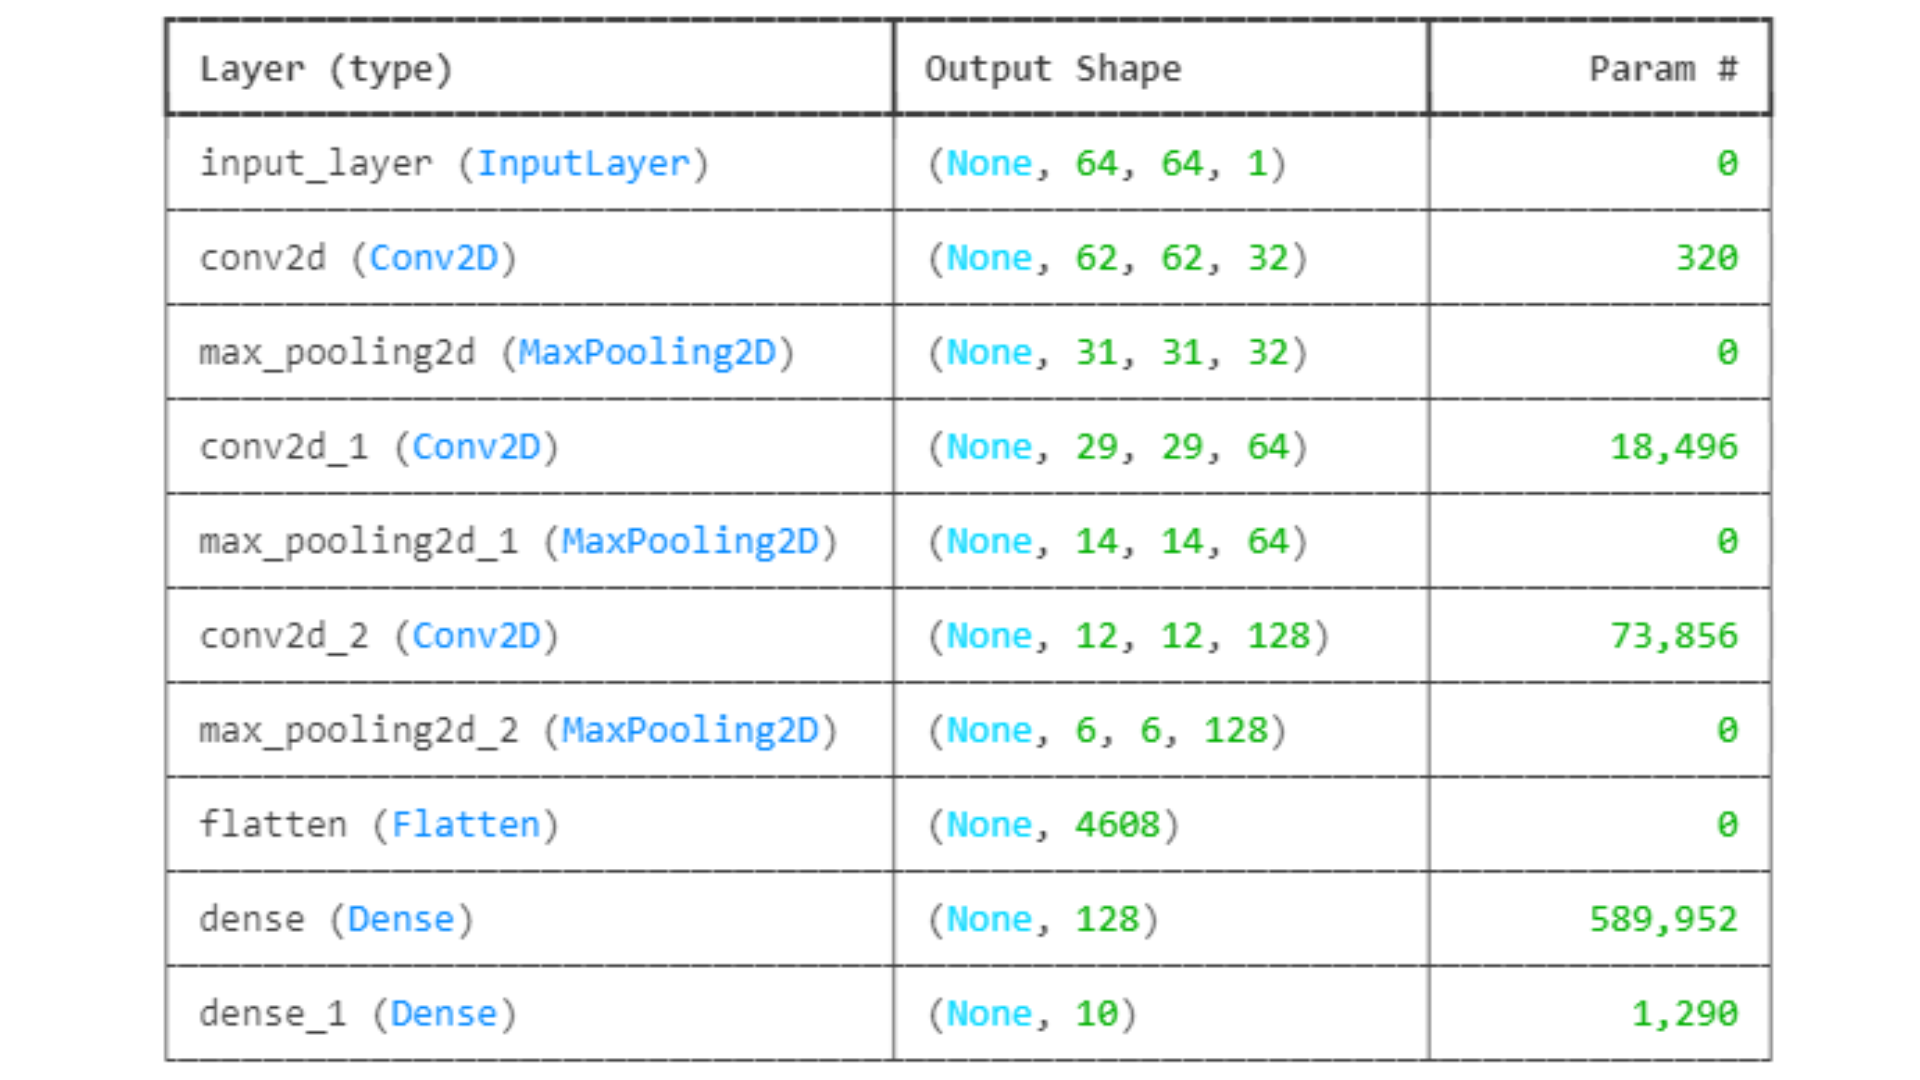
\includegraphics[width=0.75\textwidth]{imgs/p2_parameters.png}
\caption{Required Parameters for the Proposed Architecture.}\label{fig:p2Para}
\end{figure}
\subsubsection{Model Development}
This project comprises two Python scripts. The first script,\texttt{ `mmdigits.py'}, is responsible for extracting images from the specified data path and generating a substantial dataset along with a corresponding label vector, denoted as $X$ and $y$, respectively. The matrix X is formed as a large array of size $N x (64 x 64 x 1)$, where each row represents an individual image. Concurrently, the label vector $y$, with dimensions $Nx1$, contains the label for each corresponding row (or image) in $X$.

ဤ project တွင် ပါ၀င်သည့် code များကို Python file နှစ်ခုဖြင့် ပေးထားသည်။ ပထမ script \texttt{ `mmdigits.py'} တွင်  image များကို matrix အဖြစ် ဖန်တီခြင်းနှင့်၊  label များကို vector $y$ အဖြစ် တည်ဆောက်ခြင်း တို့ ပါ၀င်သည်။ ဒုတိယ script \texttt{HandDigit.ipynb} သည် အဓိက script ဖြစ်ပြီး deep learning model တည်ဆောက်ခြင်း၊ model ကို train ခြင်း နှင့် testing ပြုလုပ်ခြင်းတို့အပြင် ရလဒ်များကို သိမ်းဆည်းသည့် အပိုင်းတို့ ပါ၀င်သည်။ Python code များဖြစ်သည့်အတွက် မြန်မာ ဘာသာပြန်ဆိုခြင်း မပြုထားပါ။ 

\begin{solution}
\begin{lstlisting}
import os
import cv2
import numpy as np
def load_dataset(dataset_dir):
    images = []
    labels = []
    desired_width = 64
    desired_height = 64
    top_crop = 20
    bottom_crop = 20
    left_crop = 50
    right_crop = 50    
    # Loop through each subfolder in the dataset directory
    for class_label in os.listdir(dataset_dir):
        class_dir = os.path.join(dataset_dir, class_label)          
        # Check if it's a directory
        if os.path.isdir(class_dir):
            # Get the class label from the subfolder name
            label = int(class_label)
            # Loop through each image file in the subfolder
            for filename in os.listdir(class_dir):
                image_path = os.path.join(class_dir, filename)     
                # Read the image and convert it to grayscale
                image = cv2.imread(image_path, cv2.IMREAD_GRAYSCALE)
                # Crop and Resize image to a fixed size 
                image = image[top_crop:image.shape[0]-bottom_crop, 
                                    left_crop:image.shape[1]-right_crop]
                image = cv2.resize(image, (desired_width, desired_height))                
                # Add the image and label to the lists
                images.append(image)
                labels.append(label)

    # Convert lists to NumPy arrays
    images = np.array(images)
    labels = np.array(labels)    
    return images, labels
\end{lstlisting}  
\end{solution}

The second script, \texttt{HandDigit.ipynb}, is responsible for developing, training, and testing the deep learning model, as well as saving the results. 
In this script, two customized functions are first defined. The first function, \texttt{create\_cnn\_model(input\_shape)}, constructs the proposed architecture. The second function,\texttt{ save\_results} is responsible for saving the resulted confusion matrix and images. 

\begin{solution}
\begin{lstlisting}
def create_cnn_model(input_shape):    
    # Create an Input layer
    inputs = Input(shape=input_shape)    
    
    # Add convolutional layers
    x = Conv2D(32, kernel_size=(3, 3), activation='relu')(inputs)
    x = MaxPooling2D(pool_size=(2, 2))(x)
    x = Conv2D(64, kernel_size=(3, 3), activation='relu')(x)
    x = MaxPooling2D(pool_size=(2, 2))(x)
    x = Conv2D(128, kernel_size=(3, 3), activation='relu')(x)
    x = MaxPooling2D(pool_size=(2, 2))(x)    
    # Flatten the output from the convolutional layers
    x = Flatten()(x)    
    # Add fully connected layers
    x = Dense(128, activation='relu')(x)
    outputs = Dense(10, activation='softmax')(x)
    
    # Create the model
    model = Model(inputs=inputs, outputs=outputs)
    # Compile the model
    model.compile(optimizer='adam', loss='categorical_crossentropy', 
                        metrics=['accuracy'])   
    return model
\end{lstlisting}  
\end{solution}

\begin{solution}
\begin{lstlisting}
def save_results(y_test, y_pred, X_test, file_path):    

    result_conf  = confusion_matrix(y_test.argmax(axis=1), y_pred.argmax(axis=1))
    result_conf = pd.DataFrame(result_conf)
    result_conf.to_csv(file_path + 'cm.csv', index=False)    
    result_df = pd.DataFrame({'Test': y_test.argmax(axis=1), 
                                                'Pred': y_pred.argmax(axis=1)})
    result_df.to_csv(file_path + 'result.csv', index=False)  
    
    # Display the first image in the testing set
    idx = np.random.randint(0, X_test.shape[0])
    plt.imshow(X_test[idx], cmap='gray')
    plt.axis('off')
    plt.title(f"Predicted as: {y_pred[idx].argmax()} 
                            with percentage of {y_pred[idx].max()*100:.0f}%")
    num = y_test[idx].argmax()
    plt.savefig(file_path + str(num) + '.png', dpi = 100, bbox_inches = 'tight')
    plt.show()
\end{lstlisting}  
\end{solution}

Next, we explain the steps for developing and deploying the proposed deep learning model to classify the images into 10 different digits.
\setcounter{stepcounter}{0}
\begin{step}
The first step imports the required libraries, including the module customized module \texttt{`mmdigits'}. 
\begin{lstlisting}
from tensorflow import keras
from keras.datasets import mnist
from keras.models import Sequential, Model
from keras.utils import to_categorical, plot_model
from keras.layers import Input, Conv2D, MaxPooling2D, Flatten, Dense
from sklearn.metrics import confusion_matrix

import pydot, os
import pandas as pd
import numpy as np
import matplotlib.pyplot as plt
import mmdigits
from sklearn.model_selection import train_test_split
\end{lstlisting}  
\end{step}

\begin{step}
The second step creates a dataset for the images in the given directory using a function from the customized module \texttt{mmdigits}. This step generates a matrix, \texttt{images}, with a size of $N \times (64 \times 64)$, and a label vector, \texttt{labels}, with dimensions $N \times 1$, where each element corresponds to the label for each row (or image) in the \texttt{images} matrix. For the \texttt{Myanmar digits dataset}, $N$ is 2,200. The variable \texttt{`width'} and '\texttt{height}' decides the required image size for the proposed model. 

\begin{lstlisting}
dataset_dir = "./dataset/MM_digits/"
width = 64
height = 64
# Load the dataset
images, labels = mmdigits.load_dataset(dataset_dir)
\end{lstlisting}  
\end{step}

\begin{step}
Step 3 preprocesses the dataset. This step involves three key actions:
\begin{itemize}[b]
    \item The \texttt{images} matrix is reshaped to have dimensions $N \times (64 \times 64 \times 1)$, where each image is scaled to have pixel values between 0 and 1 by dividing by 255.0.
    \item The \texttt{labels} vector is converted to a one-hot encoded format using \texttt{keras.utils.to\_categorical}, which is essential for the classification task where the output layer has 10 neurons, one for each digit class.
    \item The dataset is then split into training and testing sets using \texttt{train\_test\_split}, with 30\% of the data allocated for testing and a random seed set for reproducibility.
\end{itemize}

\begin{lstlisting}
images = images.reshape(-1, width, height, 1).astype("float32") / 255.0
labels = keras.utils.to_categorical(labels, num_classes=10)
X_train, X_test, y_train, y_test = train_test_split(images, labels, 
                                                test_size=0.3, random_state=42)
\end{lstlisting}  
\end{step}

\begin{step}
Step 4 involves the training of the deep learning model.
\begin{lstlisting}
input_shape = (width,height,1)
model = create_cnn_model(input_shape)
model.fit(X_train, y_train, batch_size=128, epochs=10, validation_split=0.1, verbose=0)
y_pred = model.predict(X_test)
test_loss, test_accuracy = model.evaluate(X_test, y_test)
\end{lstlisting}  

\begin{itemize}[b]
    \item \texttt{input\_shape = (width,height,1)}: This line defines the input shape of the images for the model, which is required when constructing the convolutional neural network (CNN).
    \item \texttt{model = create\_cnn\_model(input\_shape)}: This line creates the CNN model using the previously defined function \texttt{create\_cnn\_model}, with the specified input shape.
    \item \texttt{model.fit(X\_train, y\_train, batch\_size=128, epochs=10, validation\_split=0.1, verbose=0)}: This line trains the model using the training data \texttt{X\_train} and labels \texttt{y\_train}. It specifies parameters such as batch size (128), number of epochs (10), validation split (10\% of training data), and verbosity level (0 for silent mode).
    \item \texttt{y\_pred = model.predict(X\_test)}: This line predicts the labels for the test data \texttt{X\_test} using the trained model.
    \item \texttt{test\_loss, test\_accuracy = model.evaluate(X\_test, y\_test)}: This line evaluates the performance of the model on the test data \texttt{X\_test} and corresponding labels \texttt{y\_test}. It returns the test loss and accuracy.
\end{itemize}
\end{step}

\begin{step}
Step 5 involves saving the results of the model evaluation. The first line specifies the directory path where the results will be saved. If the directory doesn't exist, it will be created by the second and third line by calling the \texttt{os.makedirs()} function under the \texttt{\textbf{os }}module. The last line saves the results of the model evaluation using the previously defined function \texttt{save\_results()}.  
\begin{lstlisting}
file_path = './results/mmdigit/'
if not os.path.exists(file_path):
    os.makedirs(file_path)
save_results(y_test, y_pred, X_test, file_path)
\end{lstlisting}  
\end{step}

\newpage
\subsubsection{Results and Discussion}

Figure \ref{fig:p2resutls} displays sample results of the model's predictions. The top row showcases correct predictions, accompanied by their corresponding confidence scores (probabilities). Conversely, the bottom row demonstrates instances where the model commonly misclassifies certain digits, such as 1 as 0, 0 as 8, 9 as 6, and 7 as 2.

အောက်ပါ ပုံတွင် proposed method ကို အသုံးပြု၍ ရရှိသည့် ရလဒ်များကို တင်ပြထားပါသည်။ ပထမ row တွင် အဖြေမှန်သည့် ရလဒ်များကို တင်ပြ၍ ဒုတိယ row မှားယွင်းသည့် ရလဒ်များကို ပြသထားသည်။ ဒုတိယ row၏ ပထမ ဆုံး နံပါတ်တွင် နံပါတ် \texttt{၁} ကို \texttt{၀} အဖြစ် လည်းကောင်း၊ ဒုတိယ ပုံတွင် \texttt{၀} ကို \texttt{၈} အဖြစ် လည်းကောင်း ၊ တတိယပုံတွင် \texttt{၉} ကို \texttt{၆} အဖြစ် လည်းကောင်း၊ နောက်ဆုံး ပုံတွင် \texttt{၇} ကို \texttt{၂ } အဖြစ် လည်းကောင်း မှားယွင်း ခန့်မှန်းထားသည်ကို တွေ့နိုင်သည်။ 

\vspace{0.5em}
\begin{figure}[h]%
\centering 
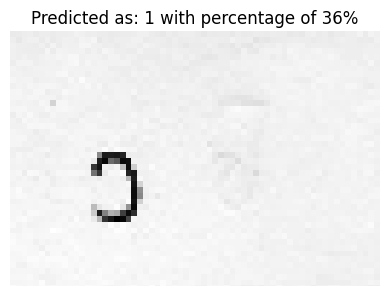
\includegraphics[width=0.225\textwidth]{imgs/1.png}
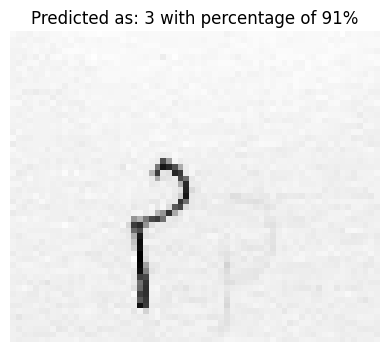
\includegraphics[width=0.22\textwidth]{imgs/3.png}
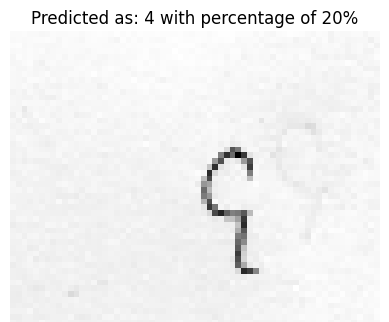
\includegraphics[width=0.225\textwidth]{imgs/4.png}
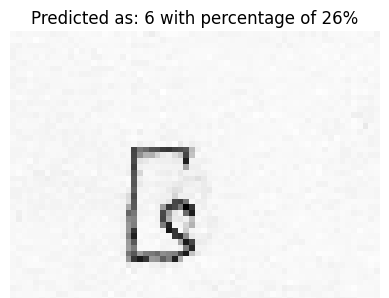
\includegraphics[width=0.225\textwidth]{imgs/6.png}
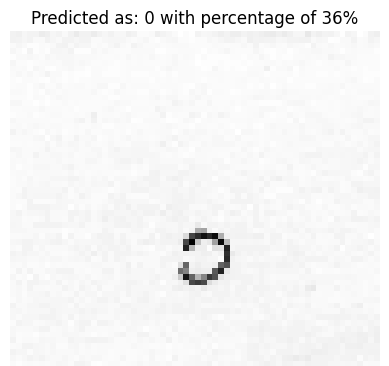
\includegraphics[width=0.225\textwidth]{imgs/1_0.png}
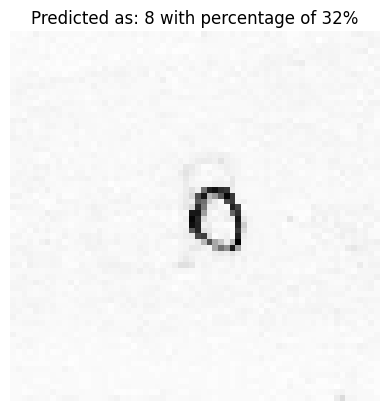
\includegraphics[width=0.22\textwidth]{imgs/0_8.png}
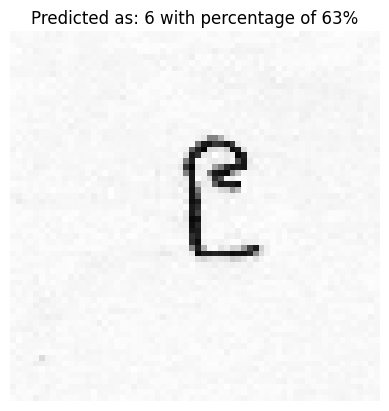
\includegraphics[width=0.22\textwidth]{imgs/9_6.png}
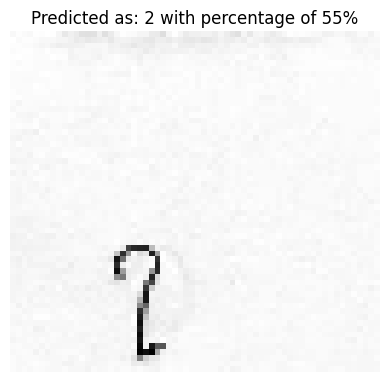
\includegraphics[width=0.225\textwidth]{imgs/7_2.png}
\caption{Sample Results of Myanmar Digits Recognition: Correct predictions (top) and incorrect predictions (bottom).}
\label{fig:p2resutls}
\end{figure}

\begin{figure}[h]
    \centering    
    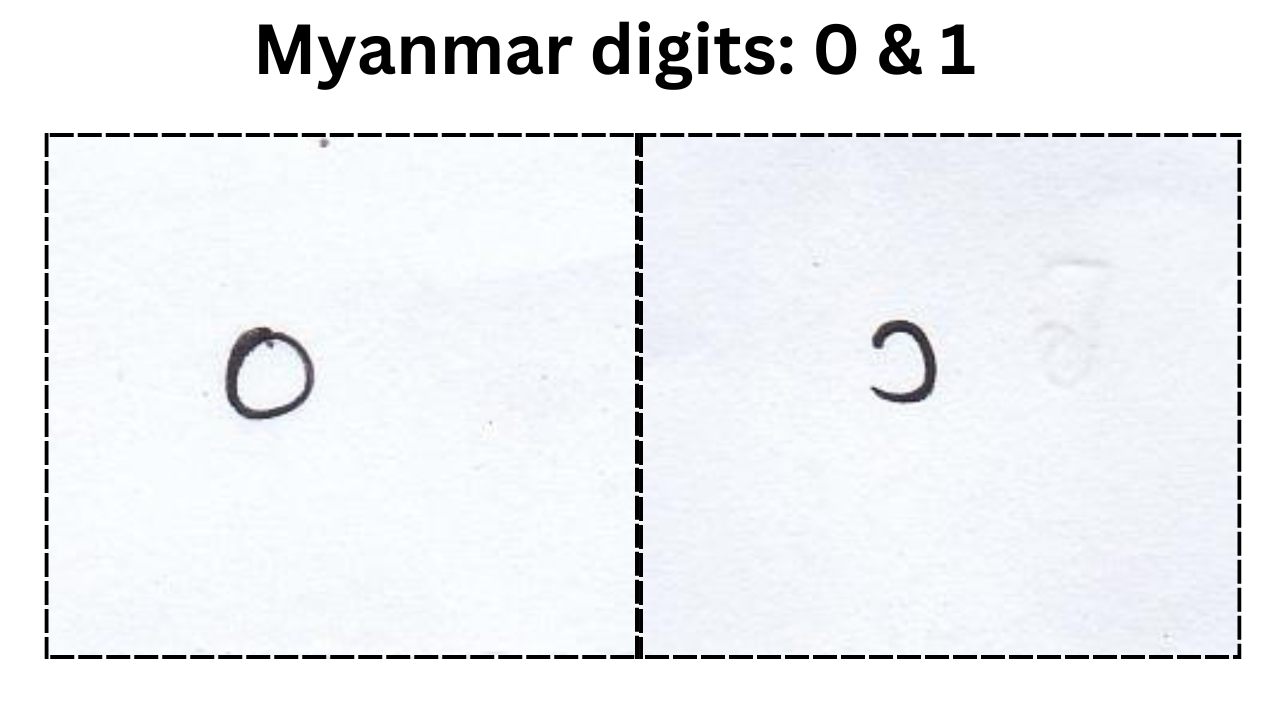
\includegraphics[width=0.45\textwidth]{imgs/0and1.png}
    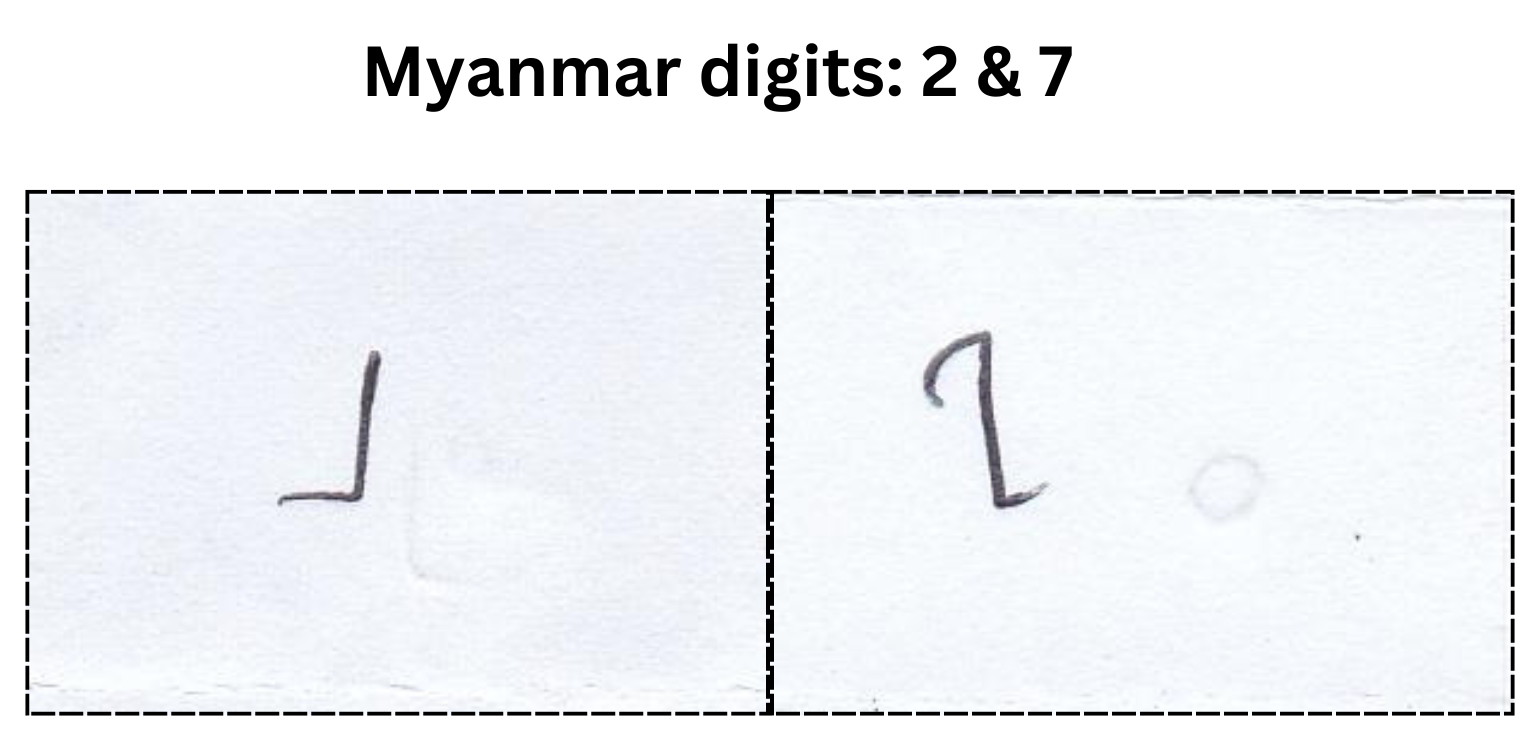
\includegraphics[width=0.5\textwidth]{imgs/2and7.png}
    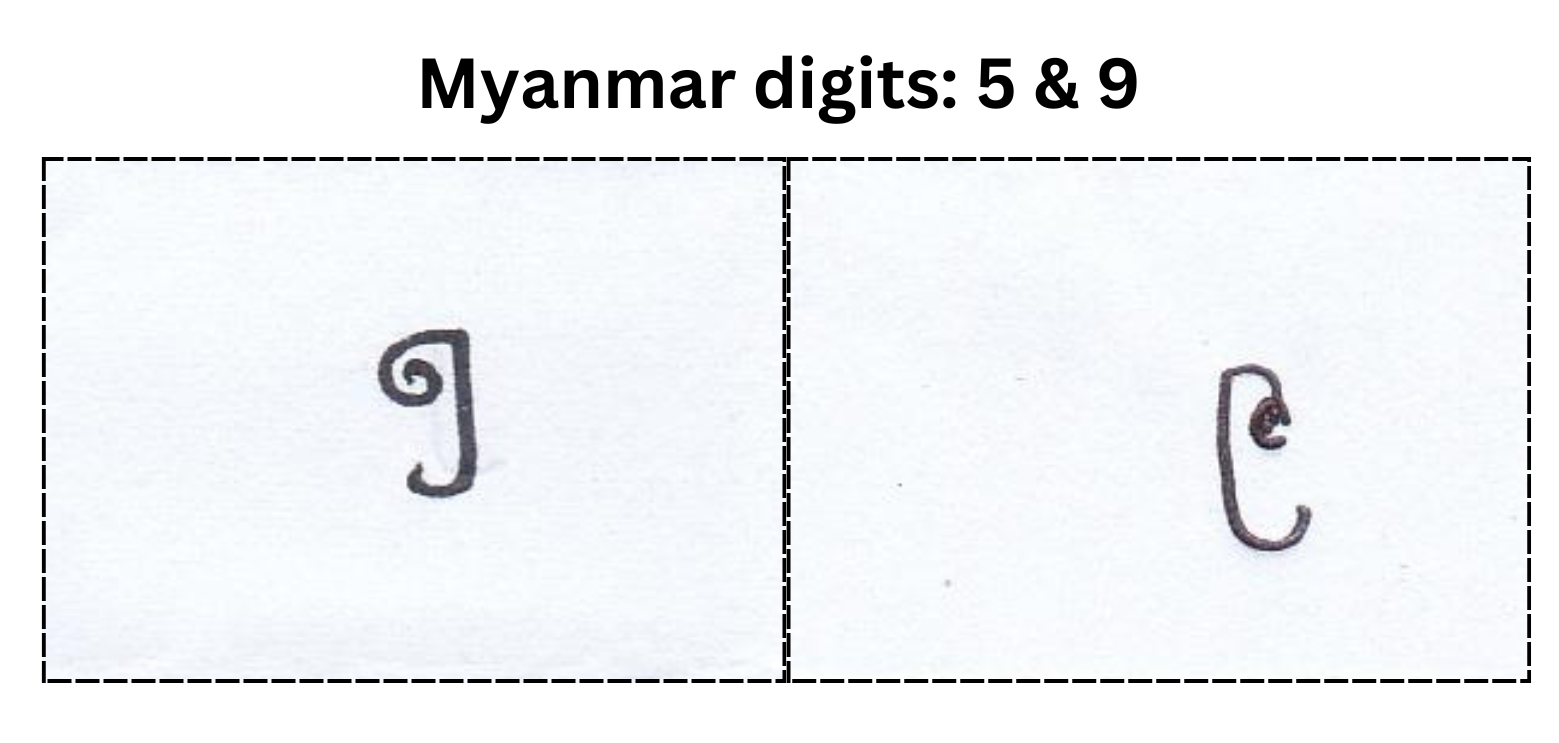
\includegraphics[width=0.45\textwidth]{imgs/5and9.png}
    \caption{Similarity between Myanmar digits `0' \& `1',  `2' \& '7', and '5' \& `9'.}
    \label{fig:mm_digits_similarity}
\end{figure}

ဤသို့ မှားယွင်း ခန့်မှန်းရသည့် အကြောင်းရင်းမှာ မြန်မာ နံပါတ်များ၏ ဆင်တူမှု ကြောင့်ဖြစ်သည်။ မြန်မာ နံပါတ်များတွင် သုည နှင့် တစ်သည် လက်ရေးသော့သူ ဖြစ်ပါက ခွဲခြားရန် ခက်ခဲသည်ကို အထက်ပါပုံတွင် တွေ့နိုင်ပါသည်။ ထို့အပြင် \texttt{၉} ၊  \texttt{၆} နှင့် \texttt{၅} တို့သည်လည် ပြောင်းပြန် လှည့်လိုက်ပါက လက်ရေးမူတွင် ထပ်တူ နီးပါး ကျနေသည်ကို တွေ့နိုင်သည်။ အောက်ပါ ဇယားတွင် testing result အတွက် ရရှိသည့် confusion matrix ကို ပြသထားပါသည်။ ပထမ row ကို ကြည့်မည်ဆိုပါက သုညကို ရှစ် အဖြစ် မှားယွင်းခန့်မှန်းထားသည့် အကြိမ်ပေါင်း နှစ်ဆယ့်ကိုး ကြိမ် ရှိသည်ကို တွေ့နိုင်ပါသည်။ သုညကို တစ်အဖြစ် မှားယွင်းမှုသည် လေး ကြိမ်သာ ဖြစ်ခဲ့သော်လည်း တစ်ကို သုည အဖြစ် မှားယွင်းမှုသည် အကြိမ် နှစ်ဆယ် ခန့် ရှိသည်ကို တွေ့ နိုင်သည်။ accuracy score မှာ ၆၀ ရာခိုင်နှုန်း ရရှိရာ ယေဘူယျ အားဖြင့် ရလဒ်သည် မဆိုးဟု ဆိုနိုင်သော်လည်း ပိုမို ကောင်းမွန်သည့် ရလဒ်များကို ရရှိနိုင်ရန် လိုအပ်နေသေးသည်။ 

Table \ref{tab:p2cm} presents the confusion matrix for the MM digits dataset. Each row represents the true label of the samples, while each column represents the predicted label by the proposed model. Notably, certain digits such as '0' and '1', as well as '6' and '9', are frequently misclassified, leading to overall accuracy score of 60\%. This is likely due to the similarities between these digits in handwritten Myanmar script, as illustrated in Figure \ref{fig:mm_digits_similarity}. 

\vspace{0.5em}
\begin{table}[h]
    \centering
    \begin{tabular}{|*{11}{c|}}
        \hline 
        & 0 & 1 & 2 & 3 & 4 & 5 & 6 & 7 & 8 & 9 \\
        \hline
        0 & \colorbox{yellow}{25} & 4 & 1 & 1 & 1 & 0 & 0 & 2 & 29 & 2 \\\hline
        1 & 20 & \colorbox{yellow}{35} & 3 & 5 & 0 & 0 & 0 & 2 & 10 & 2 \\\hline
        2 & 1 & 4 & \colorbox{yellow}{59} & 6 & 1 & 0 & 0 & 0 & 1 & 0 \\\hline
        3 & 0 & 4 & 1 & \colorbox{yellow}{45} & 9 & 0 & 1 & 1 & 0 & 1 \\\hline
        4 & 0 & 1 & 1 & 12 & \colorbox{yellow}{37} & 0 & 3 & 5 & 0 & 1 \\\hline
        5 & 0 & 0 & 1 & 2 & 12 & \colorbox{yellow}{18} & 4 & 9 & 3 & 13 \\\hline
        6 & 2 & 1 & 0 & 1 & 1 & 0 & \colorbox{yellow}{40} & 2 & 4 & 4 \\\hline
        7 & 0 & 2 & 0 & 2 & 10 & 0 & 2 & \colorbox{yellow}{50} & 1 & 2 \\\hline
        8 & 17 & 1 & 0 & 1 & 0 & 0 & 3 & 1 & \colorbox{yellow}{45} & 5 \\\hline
        9 & 1 & 3 & 1 & 9 & 1 & 0 & 8 & 4 & 1 & \colorbox{yellow}{43} \\
        \hline
    \end{tabular}
    \caption{Confusion matrix for Myanmar Handwritten digits recognition}
    \label{tab:p2cm}
\end{table}


In future work, efforts could focus on enhancing the model's performance by addressing the challenges observed in the confusion matrix presented in Table 
\ref{tab:p2cm}. Specifically, attention could be given to addressing the challenges posed by the similarities between certain digits in the handwritten Myanmar script, as illustrated in Figure \ref{fig:mm_digits_similarity}. One possible avenue for future work is collecting additional training data for these digits and augmenting the dataset with variations in handwriting styles. Additionally, fine-tuning hyperparameters and exploring alternative neural network architectures tailored to capture the intricacies of handwritten Myanmar script could be beneficial.

လက်ရေးဖြင့် ရေးထားသည့် မြန်မာ နံပါတ်များကို recognize ပြုလုပ်ခြင်းသည် မြန်မာ နည်းပညာလောက ပိုမို တိုးတက်စေရန် အရေးကြီးသည့် Project တစ်ခု ဖြစ်ပါသည်။ ယခု သင်ခန်းစာတွင် စာဖတ်သူများ အတွက် လွယ်ကူစေရန် ရိုးရှင်းသည့် deep learning model တစ်ခုကို အသုံးပြု၍ ရလဒ်များကို တင်ပြထားသော်လည်း ပိုမို ကောင်းမွန်သည့် model များကို တီထွင်သင့်ပါသည်။ ရလဒ်ကောင်းများ ရရှိနိုင်စေရန် လက်ရေး အမျိုးမျိုး ဖြင့် ရေးသားထားသည့် ဒေတာများကို ထပ်မံ စုဆောင်းခြင်း၊ model ၏ architecture ကို ပိုမိုကောင်းမွန်အောင် ပြုလုပ်ခြင်းများ ပြုလုပ်ရန် တိုက်တွန်းအပ်ပါသည်။ 

\newpage
\section{Chapter-End Exercises}\label{sec:exercises}
\begin{question}
What is one of the primary benefits of using deep learning networks over traditional (shallow) neural networks?
\begin{enumerate}[a] % Alphabetical enumeration
    \item Reduced computational resources needed for training
    \item Ability to learn hierarchical representations of data
    \item Easier to interpret and understand    
\end{enumerate}
\end{question} 

\begin{answer}
The correct answer is \texttt{Ability to learn hierarchical representations of data}. Deep learning networks excel at learning hierarchical representations of data, allowing them to capture complex patterns and features that may not be easily discernible with traditional neural networks.
\end{answer}

\begin{question}
What is the primary function of the pooling layer in a Convolutional Neural Network (CNN)?
\begin{enumerate}[a]
\item To increase the spatial dimensions of the feature maps
\item To reduce the spatial dimensions of the feature maps
\item To adjust the weights connecting the hidden layer to the output layer
\end{enumerate}
\end{question} 

\begin{question}
Which layer in a CNN connects every neuron in one layer to every neuron in the next layer, similar to traditional artificial neural networks?
\begin{enumerate}[a]
\item Input Layer
\item Convolutional Layer
\item Fully Connected Layer
\end{enumerate}
\end{question}

\begin{question}
What is the role of the output layer in a CNN for a classification task?
\begin{enumerate}[a]
\item To produce a continuous output value
\item To learn hierarchical representations of data
\item To represent the probability of the input belonging to each class
\end{enumerate}
\end{question} 